%%%%%%%%%%%%%%%%%%%%%%%%%%%%%%%%%%%%%%%%%%%%%%%%%%%%%%%%%%%%%%%%%%%%%%%%%%%%%%%%
%%%%%%%%%%%%                THIS IS THE                           %%%%%%%%%%%%%%
%%%%%%%%%%%%     ACTUS TECHNICAL SPECIFICATION DOCUMENT           %%%%%%%%%%%%%%
%%%%%%%%%%%%                   v1.0                               %%%%%%%%%%%%%%
%%%%%%%%%%%%              ----------------                        %%%%%%%%%%%%%%
%%%%%%%%%%%%        Copyright (C) 2016 - present by               %%%%%%%%%%%%%%
%%%%%%%%%%%%      ACTUS Financial Research Foundation             %%%%%%%%%%%%%%
%%%%%%%%%%%%             -----------------                        %%%%%%%%%%%%%%
%%%%%%%%%%%%      Please see distribution for license             %%%%%%%%%%%%%%
%%%%%%%%%%%%%%%%%%%%%%%%%%%%%%%%%%%%%%%%%%%%%%%%%%%%%%%%%%%%%%%%%%%%%%%%%%%%%%%%

\documentclass[9pt,oneside]{amsart}
\usepackage{multicol}
\usepackage[a4paper,
            width=170mm,
            top=18mm,
            bottom=22mm,
            includeheadfoot]{geometry}
\usepackage[bookmarks=true, 
            unicode=true, 
            pdftitle={ACTUS Technical Specification}, 
            pdfauthor={ACTUS Financial Research Foundation},
            pdfkeywords={ACTUS, Financial Contracts, Algorithmic Contracts, Technical Specification},
            pdfborder={0 0 0.5 [1 3]}]{hyperref}


% ---------------------- Language --------------------------------
\usepackage[english]{babel}


% ---------------------- floats and figures --------------------------------
\usepackage{graphicx}
\usepackage{float}
\usepackage{longtable}


% ---------------------- math --------------------------------
\usepackage{amsmath}
\usepackage{amssymb}
\usepackage{amsthm} % for theorem-style environments
\newtheorem{example}{Example}


% ------------------- special tables -----------------------------
\newenvironment{states}[1]{
	\begin{longtable}[H]{| p{0.05\textwidth} | p{0.48\textwidth} |  p{0.43\textwidth} |}
	\multicolumn{3}{c}{\textbf{#1: State Variables Initialization}}\\
	\hline
	\textbf{State} & \textbf{Initialization per $t_0$} & \textbf{Comments} \\
	\hline
	\endfirsthead
	\multicolumn{3}{c}{\textit{Continued from previous page}} \\
	\hline
	\textbf{State} & \textbf{Initialization per $t_0$} & \textbf{Comments} \\
	\hline
	\endhead
	\hline \multicolumn{3}{r}{\textit{Continued on next page}} \\
	\endfoot
	\hline
	\endlastfoot
}{%
	\hline
	\end{longtable}
}

\newenvironment{schedule}[1]{
	\begin{longtable}[H]{| p{0.05\textwidth} | p{0.5\textwidth} |  p{0.4\textwidth} |}
	\multicolumn{3}{c}{\textbf{#1: Contract Schedule}}\\
	\hline
	\textbf{Event} & \textbf{Schedule} & \textbf{Comments} \\
	\hline
	\endfirsthead
	\multicolumn{2}{c}{\textit{Continued from previous page}} \\
	\hline
	\textbf{Event} & \textbf{Schedule} & \textbf{Comments} \\
	\hline
	\endhead
	\hline \multicolumn{2}{r}{\textit{Continued on next page}} \\
	\endfoot
	\hline
	\endlastfoot
}{%
	\hline
	\end{longtable}
}

\newenvironment{functions}[1]{
    	\begin{longtable}[H]{| p{0.05\textwidth} | p{0.42\textwidth} |  p{0.48\textwidth} |}
	\multicolumn{3}{c}{\textbf{#1: State Transition Functions and Pay Off Functions}}\\
	\hline
	\textbf{Event} & \textbf{Pay Off Function} & \textbf{State Transition Function}\\
	\hline
	\endfirsthead
	\multicolumn{2}{c}{\textit{Continued from previous page}} \\
	\hline
	\textbf{Event} & \textbf{Pay Off Function} & \textbf{State Transition Function}\\
	\hline
	\endhead
	\hline \multicolumn{2}{r}{\textit{Continued on next page}} \\
	\endfoot
	\hline
	\endlastfoot
}{%
	\hline
    	\end{longtable}
}

% ---------------------- misc --------------------------------
\usepackage{verbatim}
\usepackage{natbib}
\setlength\parindent{0pt}
\newcommand{\Real}{\mathbb{R}}
\newcommand{\svar}[2]{\textbf{#1}_{#2}}
\newcommand{\attr}[1]{\texttt{#1}}
\newcommand{\stf}[2]{STF\_#1\_#2()}
\newcommand{\pof}[2]{POF\_#1\_#2()}
\newcommand{\dfl}[1]{D(\textbf{Prf}_{#1})}
\newcommand{\sgn}{R(\attr{CNTRL})}
\newcommand{\sdl}[3]{S(#1,#2,#3)}
\newcommand{\yfr}[2]{Y(#1,#2)}
\newcommand{\yfrfunc}{Y}
\newcommand{\ann}[5]{A(#1,#2,#3,#4,#5)}
\newcommand{\obs}[3]{O^{#1}(#2,#3)}
\newcommand{\obsfull}[5]{O^{#1}(#2,#3,#4,#5)}
\newcommand{\obsfunc}[1]{O^{#1}}
\newcommand{\uly}[3]{U(#1,#2,#3)}
\newcommand{\undef}{\varnothing}
\newcommand{\tmax}{t^{max}}


% ---------------------- Input options --------------------------------
\newcommand{\VersionNumber}{unknown revision}
\IfFileExists{build_options.tex}{\input{build_options.tex}}


%%%%%%%%%%%%%%%%%%%%        Titlepage          %%%%%%%%%%%%%%%%%%%%

\title{ACTUS: The algorithmic representation of financial contracts \\
      {\smaller \textbf{Version \VersionNumber}}}

\author{
    ACTUS Financial Research Foundation\\
    info@actusfrf.org
}

%%%%%%%%%%%%%%%%%%%% Document code starts here %%%%%%%%%%%%%%%%%%%%

\begin{document}

%\begin{abstract}
%
%\end{abstract}

\maketitle



%%%%%%%%%%%%%%%%%%%  About  %%%%%%%%%%%%%%%%%%%%

\section*{About this document}\label{sec:about}

This Document defines provides high-level documentation regarding the Algorithmic Contract Types Unified Standards (ACTUS).  It is provided to the ACTUS Users Association by the ACTUS Financial Research Foundation under the terms of the open source, public good contribution of the ACTUS body of work by the ACTUS Financial Research Foundation.


%%%%%%%%%%%%%%%%%%%%  Versions  %%%%%%%%%%%%%%%%%%%%

\section*{Versions}\label{sec:version}

The version of this document (cf. titlepage) has following format: [major].[minor]-[revision]-[date] where [major] and [minor] are integers marking major and minor release, [revision] indicates an unreleased revision in form of the short form of the respective git commit hash, and [date] the respective date of the revision. Releases are recorded in the following table with minor releases increasing the version number by 0.1; major releases by 1.0.

\begin{table}[H]
  \centering
  \begin{tabular}{| p{0.1\textwidth} | p{0.1\textwidth} | p{0.75\textwidth} |}
  \hline
  Date & Version & Description \\ 
  \hline
  2016-06-17 & 0.1 & Initial Draft of the ACTUS High Level Description \\
  \hline
  2017-04-06 & 0.2 & Various conceptual refinements, introduced PP (Principal Prepayment), and PY   (Penalty Payment) event types, introduced Contract Types Call Money (CLM), Cash (CSH), Commodity (COM), Foreign Exchange Outright (FXOUT) \\
  \hline
  2018-09-30 & 1.0 & General overhaul of the specifications including introduction of various interfaces, additional rate-reset related attributes and Undefined Maturity Profile (UMP) Contract Type.\\
  \hline
  \end{tabular}
\end{table}


%%%%%%%%%%%%  Starting new page here %%%%%%%%%%%%%%

\newpage


%%%%%%%%%%%%  Table Of Contents %%%%%%%%%%%%%%

\tableofcontents


%%%%%%%%%%%%  Starting new page here %%%%%%%%%%%%%%

\newpage


%%%%%%%%%%%%%%%%%%%% 2-columns starts here %%%%%%%%%%%%%%%%%%%%
\setlength{\columnsep}{20pt}
\begin{multicols}{2}


%%%%%%%%%%%%%%%%%%%%  Introduction  %%%%%%%%%%%%%%%%%%%%

\section{Introduction}\label{sec:intro}

Financial contracts are legal agreements between two (or more) counterparties on the exchange of future cash flows. Such legal agreements are defined unambiguously by means of a set of contractual terms and logic. As a result, financial contracts can be described mathematically and represented as computer readable algorithms.

The exchange of cash flows between counterparties follows certain patterns. Each pattern is called ContractType (CT) within the ACTUS framework. A typical CT or exchange pattern of cash flows is what we could call the bond pattern where principal is exchanged initially followed by a period of cyclical interest payments and finally the principal is reversed at maturity date. Interest rates could be fixed or variable with certain interest rate reset cycles. This pattern is used also for many types of loans. Within ACTUS this CT is called PrincipalAtMaturity or PAM for short.

Another popular pattern is used for mortgages in many countries. Principal is also exchanged initially followed however by regular payments which combine interest and principal redemption at the same time. Since the total payment is given, the split between the principal portion and the interest portion varies over time. This CT is called Annuity or ANN. PAM and ANN are two examples of CT´s. As we will see below, there are about thirty CT´s to describe the overwhelming bulk of all cash flow exchange patterns found in the financial world.

Financial contracts represent the deterministic part of finance. This offers a strict definition for what belongs to a contract and what not. It especially excludes any stochastic element which are called risk factors within the ACTUS framework. ACTUS has a clearly defined interface to these risk factor (see the specific chapter below) but it does not model these risk factors. The link between ACTUS and the risk factors can best be explained with the variable side of a swap or any variable rate instrument that resets its rate periodically.

A variable rate instrument has a current coupon that is known and therefore part of the contract attributes. It also has a rule, how to derive new rates such as \textit{Libor plus x basis points}. These rules are contract terms and therefore also part of the contract attributes. However, ACTUS is agnostic towards the external market link (or Risk Factor) from which the new rate is fed upon a rate reset.


%%%%%%%%%%%%%%%%%%%%  Taxonomy  %%%%%%%%%%%%%%%%%%%%

\section{Financial contract taxonomy}

Below an overview of the ACTUS Contract Types taxonomy.


%%%%%%%%%%%%%%%%%%%% Figure/Image No: 2 starts here %%%%%%%%%%%%%%%%%%%%

\begin{figure}[H]
	\centering
	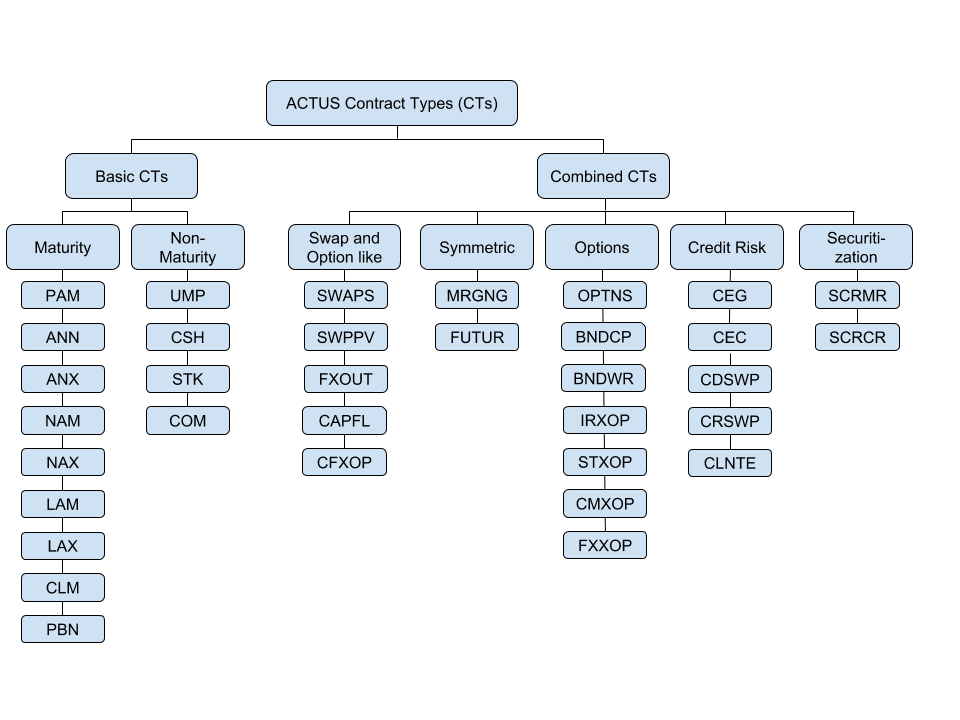
\includegraphics[width=0.45\textwidth]{./media/taxonomy.png}
	\caption{An overview of the ACTUS Contract Types Taxonomy.}
	\label{fig:taxonomy}
\end{figure}


%%%%%%%%%%%%%%%%%%%% Figure/Image No: 2 Ends here %%%%%%%%%%%%%%%%%%%%


Table \ref{tbl:taxonomy} provides further details on the ACTUS Taxonomy including the real-world financial contracts covered through the various ACTUS Contract Types.


\end{multicols}

%%%%%%%%%%%%%%%%%%%% Table No: 3 starts here %%%%%%%%%%%%%%%%%%%%


\begin{longtable}{| p{0.07\textwidth}p{0.07\textwidth}p{0.1\textwidth}p{0.45\textwidth}p{0.2\textwidth} |}
	\hline
	\textbf{Family} & \textbf{Class} & \textbf{Type} & \textbf{Description} & \textbf{Covered contracts} \\
	\hline
	\endfirsthead
	\multicolumn{4}{c}{\textit{Continued from previous page}} \\
	\hline
	\textbf{Family} & \textbf{Class} & \textbf{Type} & \textbf{Description} & \textbf{Covered contracts} \\
	\hline
	\endhead
	\hline \multicolumn{4}{r}{\textit{Continued on next page}} \\
	\endfoot
	\hline
	\endlastfoot
	Basic CT & Maturity & PAM: Principal at Maturity & Principal payment fully at Initial Exchange Date (IED) and repaid at Maturity Date (MD). Fixed and variable rates. & All kind of bonds, term deposits, bullet loans and mortgages etc. \\
	\hline
	 & & ANN: Annuity & Principal payment fully at IED and interest plus principal repaid periodically in constant amounts till MD. If variable rate, total amount for interest and principal is recalculated to be fully matured at MD. & Classical level payment mortgages, leasing contracts etc. \\
	\hline 
	 & & NAM: Negative Amortizer & Similar as ANN. However when resetting rate, total amount (interest plus principal) stay constant. MD shifts. Only variable rates. & Special class of ARM´s (adjustable rate mortgages), Certain loans. \\
	\hline 
	 & & LAM: Linear Amortizer & Principal payment fully at IED. Principal repaid periodically in constant amounts till MD. Interest gets reduced accordingly. If variable rate, only interest payment is recalculated. Fixed and variable rates. & Many amortizing loans \\
	\hline 
	 & & ANX: Exotic Annuity & Exotic version of ANN However step ups with respect to (i) Principal, (ii) Interest rates are possible. Highly flexible to match totally irregular principal payments. Principal can also be paid out in steps. & A special version of this kind are teaser rate loans and mortgages with annuity features \\
	\hline 
	 & & LAX: Exotic Linear Amortizer & Exotic version of LAM. However step ups with respect to (i) Principal, (ii) Interest rates are possible. Highly flexible to match totally irregular principal payments. Principal can also be paid out in steps. & A special version of this kind are teaser rate loans and mortgages \\
	\hline 
	 & & NAX: Exotic Negative Amortizer & Exotic version of NAM However step ups with respect to (i) Principal, (ii) Interest rates are possible. Highly flexible to match totally irregular principal payments. Principal can also be paid out in steps. & A special version of this kind are teaser rate loans and mortgages with variable MD \\
	\hline 
	 & & CLM: Call Money & Loans that are rolled over as long as they are not called. Once called it has to be paid back after the stipulated notice period. & Interbank loans with call features \\
	\hline 
	 & & PBN: Perpetual Bonds &  Bonds without any maturity date. Interest is paid into eternity if is not terminated. & Consoles, war loans \\
	\hline 
	 & Non-Maturity & UMP: Undefined Maturity Profile & Principal paid in and out at any point in time without prefixed schedule. Interest calculated on outstanding and capitalized periodically. Needs link to a behavioral function describing expected flows. & Saving products of all kind, current accounts. In some countries even variable rate mortgages can be represented with this CT \\
	\hline 
	 & & CSH: Cash & Cash or cash equivalent position & Cash, deposits at central bank \\
	\hline 
	 & & STK: Stock & Any instrument which is bought at a certain amount (market price normally) and then follows an index. & All straight stocks \\
	\hline 
	 & & COM: Commodity & This is not a financial contract in its proper sense. However it tracks movements of commodities such as oil, gas or even houses. Such commodities can serve as underlyings of commodity futures, guarantees or simply asset positions. & Oil, gas, electricity, houses etc. \\
	\hline 
	Combined & Swap and Option like & SWAPS: Swap & Exchange of two basic CT´s (PAM, ANN etc.). Normally one is fixed, the other variable. However all variants possible including different currencies for cross currency swaps, basic swaps or even different principal exchange programs. & All kind of swaps. The variety is defined by the underlying CT´s which currently are PAM and ANN in all tis flavors. With each new basic CT the variety rises \\
	\hline 
	 & & SWPPV: Plain Vanilla Swap & Plain vanilla swaps where the underlying is always a PAM and one leg is fixed, the other variable. Plain vanilla cross currency swaps also covered. & More than 90\%  of all interest rate swaps follow this simple pattern. \\
	\hline 
	 & & FXOUT: Foreign Ex-change Outright & Two parties agree to exchange two fixed cash flows in different currencies at a certain point in time in future. & Any FX-outright transaction. This is also the underlying of FX-options and FX futures \\
	\hline 
	 & & CAPFL: Cap Floors & Interest rate option expressed in a maximum or minimum interest rate & Caps and Floor options \\
	\hline 
	 & & CFXOP: Exotic Cap Floor & Exotic variants of caps and floors & \\
	\hline 
	 & Securiti-zation & SCRMR: Securitized Instruments Market Risk & Instruments bundled and traded in tranches without any specific credit risk feature & MBS, ABS, Principal only, Interest only instruments \\
	\hline 
	 & & SCRCR: Securitized instrument Credit Risk Feature & Instruments bundled and traded in tranches that include specific credit risk feature & CDOs \\
	\hline 
	 & Symmetric & MRGNG & A generic margining contract governing the agreement of margining usually present at central clearing houses & \\
	\hline 
	 & & FUTUR: Future & Keeps track of value changes for any basic CT as underlying (PAM, ANN etc. but also FXOUT, STK, COM). Handles margining calls. & Standard interest rate, FX, stock and commodity futures. \\
	\hline 
	 & Options & OPTNS: Option & Calculates straight option pay-off for any basic CT as underlying (PAM, ANN etc.) but also SWAPS, FXOUT, STK and COM. Single, periodic and continuous strike is supported. & European, American and Bermudan options with Interest rate, FX and stock futures as underlying instruments \\
	\hline 
	 & & BNDCP: Callable or puttable maturity contract & Bonds with a call or put option. If option is exercised, underlying bond ceases to exist. & Callable and puttable bonds or loans \\
	\hline 
	 & & BNDWR: Bond with warrant & Bonds with a warrant. If option is exercised, underlying bond continues to exist. & Warrants \\
	\hline 
	 & & IRXOP: Exotic Interest Rate Option & Exotic interest rate options & \\
	\hline 
	 & & STXOP: Stock Option & Exotic stock options &  \\
	\hline 
	 & & CMXOP: Exotic Commodity Option & Exotic commodity options & \\
	\hline 
	 & & FXXOP: Exotic FX Option & Exotic FX options & \\
	\hline 
	 & Credit Risk & CEG: Guarantees & Guarantee is a credit enhancement contract. It creates a relationship between a guarantor, an obligee and a debtor, moving the exposure from the debtor to the guarantor. & Personal guarantee. Government guarantee. Underlyings of CDOs. \\
	\hline 
	 & & CEC: Collateral & Collateral is a credit enhancement contract. It creates a relationship between a collateral an obligee and a debtor, covering the exposure from the debtor with the collateral. & Mortgages include a collateral contract. Any coverage with financial or physical collateral \\
	\hline 
	 & & CDSWP: Credit Default Swap & All sorts of credit default swaps &  \\
	\hline 
	 & & CRSWP: Total Return Swap & All sorts of total return swaps & \\
	\hline 
	 & & CLNTE: Credit Linked Note & All sorts of credit linked notes & \\
	\hline
	\caption{Financial contract taxonomy}
	\label{tbl:taxonomy}
\end{longtable}

%%%%%%%%%%%%%%%%%%%% Table No: 3 ends here %%%%%%%%%%%%%%%%%%%%


%%%%%%%%%%%%%%%%%%%% 2-columns starts here %%%%%%%%%%%%%%%%%%%%
\setlength{\columnsep}{20pt}
\begin{multicols}{2}


%%%%%%%%%%%%%%%%%%%% Notations %%%%%%%%%%%%%%%%%%%%

\section{Notations}\label{sec:notations}

\subsection{Contract Attributes }

Contract Attributes represent the legal contractual terms that define the exchange of cash-flows of a financial contract. Contract Attributes are introduced by the ACTUS data standard and described in the ACTUS Data Dictionary (DD). Throughout this document Contract Attributes are written in the short form and expressed in capitals (not bold). 

\begin{example}[Contract Attribute]
The ACTUS attribute \textit{Initial Exchange Date} is represented in short form \attr{IED}.
\end{example}


\subsection{$\undef$-Operator}

The $\undef$-operator is used to indicate that a certain property is undefined or, in other words, that no value has been assigned to the respective property. In particular, for optional contract attributes it means that the attribute is not defined and for schedule times (see section \ref{sec:schedules}) it means that the respective schedule is empty, i.e. no schedule time defined.

\begin{example}[Undefined Attribute]
$\attr{IPANX}=\undef$ indicates that attribute \attr{IPANX} is undefined.
\end{example}

\begin{example}[Empty Schedule]
$\vec{t}^{IP}=\undef$ means the same as $\vec{t}^{IP}=\{\}$, with $\{\}$ the empty set, and states that the IP schedule $\vec{t}^{IP}$ does not contain a schedule time.
\end{example}


\subsection{$t_0$-Time}

$t_0$ marks the time as per which the state of a contract is represented in form of the respective set of attributes. Status Date \attr{SD} itself is an attribute of the contract. In general, from the contractual logic we are able to derive any contractual events and contract states for any time $t>t_0$.


\subsection{State Variables}

State Variables describe the inner state of a financial contract at a certain point in time $t$ during its lifetime such as (outstanding) Nominal Value, applicable Interest Rate, or the contract performance through Contract Status. State Variables are written in the short form as defined in table \ref{tbl:statevars} with first letter capitalized, printed in bold, and indexed with time.

\begin{example}[State Variables]
$\svar{Nvl}{t}$ refers to the State Variable \textit{Nominal Value} observed at per time $t$.
\end{example}


\subsection{Contract Events}

A contract event $e_t^k$ refers to any contractually scheduled or un-scheduled event at a certain time $t$ and of a certain type $k$. Contract events mark specific points in time during the lifetime of a financial contract at which a cash flow is being exchanged (see section \ref{sec:pof}) or the State Variables of the contract are being updated (see section \ref{sec:stf}). Contract Events types $k$ are written in the short form as defined in table \ref{tbl:events}.

\begin{example}[Contract Events]
The \textit{Initial Exchange Date} event with event time $s$ is written as $e_s^{IED}$.
\end{example}


\subsection{State Transition Functions}

State Transition Functions (STF) define how the State Variables are being updated when a certain Contract Event applies from a pre-event state indexed $t^-$ to a post-event state indexed $t^+$. These functions are specific to a certain Contract Event and Contract Type. STFs are written according to the following pattern \stf{[event type]}{[contract type]} where [event type] and [contract type] refer to the respective event type and contract type to which the STF belongs.

\begin{example}[State Transition Functions]
The STF for an IP event and PAM contract is written as \stf{IP}{PAM} and maps e.g. state variable \textit{Nominal Accrued} from a pre-event state $\svar{Nac}{t^-}$ to post-event state $\svar{Nac}{t^+}$.
\end{example}


\subsection{Pay Off Functions}

Pay Off Functions (POF) define how the cash flow for a certain Contract Event is being derived from current State Variables and Contract Attributes. These functions are specific to a certain Contract Event and Contract Type. POFs are written according to the following pattern \pof{[event type]}{[contract type]} where [event type] and [contract type] refer to the respective event type and contract type to which the STF belongs.

\begin{example}[Pay Off Functions]
The POF for an IP event and PAM contract is written as \pof{IP}{PAM}.
\end{example}


\subsection{Date/Time}

ACTUS builds on the ISO 8601 date/time format. Hence, dates are generally expressed in the following format: [YYYY]-[MM]-[DD]T[hh]:[mm]:[ss].

Time zone information is currently not supported.

A special case is \textit{midnight}. ISO 8601 recognizes both times 00:00:00 and 24:00:00 each referring to midnight. Yet, while 24:00:00 refers to the end of one day, 00:00:00 refers to the beginning of the following day. In ACTUS the interpretation is the same why the time period (measured in any time unit) between the two points in time will always be zero. 

For brevity, we use the term \textit{time} for a specific date-time variable and in particular abbreviation Tev for the date of a Contract Event.


\subsection{Event Sequence}

Contract Events of different types may occur at the same time, i.e. exactly the same point in time. In this case, the sequence of evaluating their State Transition and Pay Off Functions is decisive for the resulting cash flows and state updates. The Event Sequence given for all events in table \ref{tbl:events} defines the order in which these functions are evaluated for the respective event types.


\subsection{Contract Lifetime}

The lifetime of an ACTUS contract is the time period of its existence from the perspective of the analyzing user. For every point in time during its lifetime, an ACTUS contract can be analyzed in terms of current State Variables and future cash flows.\\

The lifetime of a contract starts with its \attr{SD} and ends with $\min(MD, AMD, PR^*, STD, TD,\tmax)$.\\

Note that $PR^*$ refers to the PR event of a maturity contract after which \textbf{Nvl}=0.0 (i.e. at which the remaining outstanding principal is redeemed). Further, \attr{MD}, \attr{AMD}, and PR(\textbf{Nvl}=0.0) in the definition above do only apply for maturity contracts but have to be considered infinity in all other cases. Similarly, \attr{STD} only applies for certain contracts and is considered infinity for all others. Finally, $\tmax$ is a parameter that may be used to restrict the considered lifetime in an analysis. In particular, this parameter is used for contracts that do not have a \textit{natural} end to their lifetime such as STK.


%%%%%%%%%%%%%%%%%%%% Utility Functions %%%%%%%%%%%%%%%%%%%%

\section{Utility Functions}

\subsection{Schedules}\label{sec:schedules}

A schedule is a function $S$ mapping times $s,T$ with $s<T$ and cycle $c$ onto a sequence $\vec{t}$ of cyclic times

\[
	\sdl{s}{c}{T}=\vec{t}=\begin{cases} \{\} & \text{if}\quad s=\undef\land T=\undef\\ 
					s & \text{else if}\quad T=\undef\\
					(s,T) & \text{else if}\quad c=\undef\\
					(s=t_1,...,t_n=T) & \text{else} \end{cases}
\]

with $t_i<t_{i+1}, i=1,2,...$. While the schedule function can be used to create arbitrary sequences of times, it is usually used to generate sequences of cyclic events $\vec{t}^k$ of a certain type $k$, e.g. $k=IP$ for interest payment events (cf. table \ref{tbl:events}) and the following build inputs to the function

\begin{itemize}
	\item[$s$] $=k\attr{ANX}$ with $k\attr{ANX}$ attribute cycle anchor date of event type $k$
	
	\item[$c$] $=k\attr{CL}$ with $k\attr{CL}$ event type $k$'s schedule cycle
	
	\item[$T$] $=\attr{MD}$ with \attr{MD} the contract's maturity
\end{itemize}

Thereby, cycles $k\attr{CL}$ have format $NPS$ where 

\begin{itemize}
	\item[$N$] is an integer
	\item[$P$] is a time period unit (D=Day, W=Week, M=Month, Q=Quarter, H=Half Year, Y=Year)
	\item[$S$] is a \textit{stub} information ($+$=long last stub, $-$=short last stub)
\end{itemize}

Further, the last stub is defined as follows

\begin{itemize}
	\item[if] $t_{n-1}+c=T \lor S=$'-' then no stub correction applies

	\item[else] $t_n$ is removed from the schedule
\end{itemize}

The sequence of schedule times $\vec{t}^k$ may also be influenced by the \attr{EOF} and \attr{BDC} conventions and the full function syntax becomes $\sdl{s}{c}{T, \attr{EOMC}, \attr{BDC}}$. Due to such effects the sequence of schedule times can be non-equidistant or, in other words, $t_i^k-t_{i-1}^k\neq t_j^k-t_{j-1}^k, i\neq j$.\\

Note that for brevity we will omit the \attr{EOMC} and \attr{BDC} function arguments throughout this document.


\subsection{Array Schedules}

Array Schedules are defined by vector-valued inputs $\vec{s}=(s_0,s_1,...,s_m)$ and $\vec{c}=(c_0,c_1,...,c_m)$ to the regular schedule function

\begin{multline*}
	\sdl{\vec{s}}{\vec{c}}{T} = (\sdl{s_0}{c_0}{s_1-c_0},\\
					\sdl{s_1}{c_1}{s_2-c_1},...,\sdl{s_m}{c_m}{T})
\end{multline*}


Hence, array schedules are a generalization for regular schedules which coincide for $m=1$. In accordance with regular schedules \attr{EOMC} and \attr{BDC} conventions also apply here.


\subsection{End Of Month effects}

For schedules $\vec{t}^k$ starting at time $s$ which marks the end of a month with 30 or less days, e.g. April 30, and with a cycle $c$ being a multiple of 1M- attribute \attr{EOM} defines whether the schedule times are to fall on the 30th of all months (same day) or the 31st (end of month).\\ 

More specifically, \attr{EOM} has an effect on a schedule $\vec{t}^k$ only if:

\begin{itemize}
	\item[$s$] is the last day of a month with less than 31 days (Feb, April etc.)

	\item[$c$] $=NPS$ with $P\in(M, Q, H or Y)$
\end{itemize}

As per the DD \attr{EOM} can take one of the following values:
\begin{itemize}
	\item[EOM] (EndOfMonth): times $t_i,i=1,2,...,n-1$ are moved to the end of the respective months

	\item[SD] (SameDay): times $t_i,i=1,2,...,n-1$ remain unchanged except in February, where it will go to the last day if the day of month of time $s$ is higher than the number of days of February
\end{itemize}


\subsection{Business Day effects}

In general, contract events are scheduled for business days only. Therefore, the \attr{BDC} convention defines how scheduled times $t_i,i=1,2,...,n-1$ are shifted in case they fall on a non-business day:

\begin{itemize}
	\item[NULL:] No shift

	\item[SCF:] Shift/Calculate following: The event is shifted to the following non working day. Calculation of the event happens after the shift

	\item[SCMF:] Shift/Calculate modified following: The event is shifted to the following non working day. However, if the following day happens to fall into the next month, then take preceeding non-working day. Calculation of the event happens after the shift

	\item[CSF:] Calculate/Shift following: Same like SCF however calculation of the event happens before the shift

	\item[CSMF:] Calculate/Shift modified following: Same like SCMF however calculation of the event happens before the shift

	\item[SCP:] Shift/Calculate preceding: The event is shifted to the last preceding non working day. Calculation of the event happens after the shift

	\item[SCMP:] Shift/Calculate modified preceding: The event is shifted to the last preceding non working day. However, if the preceding day happens to fall into the previous month, then take next non-working day. Calculation of the event happens after the shift

	\item[CSP:] Calculate/Shift preceding: Same like SCP however calculation of the event happens before the shift

	\item[CSMP:] Calculate/Shift modified preceding: Same like SCMP however calculation of the event happens before the shift
\end{itemize}



\subsection{Business Day Function}

Whether a specific day is a business day (cf. previous section) is defined by attribute \attr{CLDR}. Such conventions generally depend on regional official holiday calendars. The Business Day Function interface allows determining for some \attr{CLDR} whether any time $t$ is a business day or not

\[
	B: t \mapsto \{true, false\}
\]

where $true$ indicates that $t$ is a business day and $false$ that it is a holiday.


\begin{example}
Two standard \attr{CLDR} implementations are the following
\begin{itemize}
	\item NoHoliday (default): every calendar day is a business day

	\item MondayToFriday: all weekdays Monday, Tuesday, Wednesday, Thursday, and Friday are business days
\end{itemize}
\end{example}


\subsection{Year Fraction Function}

Interest income and other calculations are based on \textit{per annum} interest rates. Therefore, the year-fraction function interface $Y$ is used to calculate the \textit{fraction of a year} between any two times $s$ and $t$ with $t>s$ for which e.g. an (per annum) interest rate applies according to some day count convention \attr{DCC}

\[
	\yfrfunc: s,t,\attr{DCC} \mapsto \Real
\]

Note, the year fraction function interface only defines the structure of year fraction functions but not an actual implementation thereof, or the respective \attr{DCC}, respectively. Therefore, any \attr{DCC} can be implemented according to the interface above supporting user-defined year fraction functions.\\

For brevity we will omit the \attr{DCC} function argument wherever this does not lead to confusion.


\subsection{Contract Role Sign}

The two counterparties to a financial contract are defined through attributes \attr{LEIRC} and \attr{LEICP}. The first is the party initially \textit{creating} the contract and the second is the counterparty, respectively. Thereby, both \attr{LEIRC}/\attr{LEICP} can take any \textit{role} in the contract or, more specifically, they can be the lender or borrower in a loan (PAM), fixed receiver or payer in an interest rate swap (SWAPS), etc.\\

The \textit{role} of the \attr{LEIRC} is defined through attribute \attr{CNTRL}. The \textit{role} of \attr{LEICP} is derived as the \textit{opposite} side to the contract. Apart from \attr{CNTRL} the attributes are \textit{neutral} to the \textit{role} of \attr{LEIRC} (or \attr{LEICP}).\\

On the other hand, contractual cash flows generated by the POFs and certain state variables are \textit{role-sensitive}. That is, from the perspective of the \attr{LEIRC} these quantities represent either claims or obligations. Contract Role Sign function $R$ maps the \attr{CNTRL} attribute into $+1$ indicating a claim or $-1$ indicating an obligation

\[
	R : \attr{CNTRL} \rightarrow \{-1, +1 \}
\]

When multiplying with a cash flow $x$ the Contract Role Sign function thereby defines the direction of that flow:

\begin{itemize}
	\item[$x>0$:] $x$ flows from \attr{LEICP} to \attr{LEIRC}
	
	\item[$x<0$:] $x$ flows from \attr{LEIRC} to \attr{LEICP}
\end{itemize}

Table \ref{tbl:cntrl} defines the domain of the Contract Role Sign function, i.e. the range of attribute \attr{CNTRL}, with meaning and Contract Role Sign to which the function maps.


%%%%%%%%%%%%%%%%%%%% Table No: 4 starts here %%%%%%%%%%%%%%%%%%%%


\begin{table}[H]
	\centering
	\begin{tabular}{| p{0.5in}p{1.5in}p{0.2in} |}
	\hline
	\textbf{Value} & \textbf{Meaning} & $\textbf{R}$ \\
	\hline
	RPA & Real position asset & +1 \\
	\hline
	RPL & Real position liability & -1 \\
	\hline
	CLO & Role of a collateral & +1 \\
	\hline
	CNO & Role of a close-out-netting & +1 \\
	\hline
	COL & Role of an underlying to a collateral & +1 \\
	\hline
	LG & Long position & +1 \\
	\hline
	ST & Short position & -1 \\
	\hline
	BUYER & Protection buyer & +1 \\
	\hline
	SELLER & Protection seller & -1 \\
	\hline
	RFL & Receive first leg & +1 \\
	\hline
	PFL & Pay first leg & -1 \\
	\hline
	RF & Receive fix leg & +1 \\
	\hline
	PF & Pay fix leg & -1 \\
	\hline
	\end{tabular}
	\caption{Contract Role definitions.}
	\label{tbl:cntrl}
\end{table}


%%%%%%%%%%%%%%%%%%%% Table No: 4 ends here %%%%%%%%%%%%%%%%%%%%


\subsection{Contract Default Convention}

Performance of a contract indicates whether as per a certain time all parties involved adhere to their obligations arising from the contract. Attribute \attr{CTS} captures a contract's performance as per $t_0$. For any time $t>t_0$ and depending on the behavior of the parties involved the contract can migrate into different contract (performance) statuses from \textit{'performing'} to \textit{'default'}. State variable $\svar{Prf}{t}$ (cf. table \ref{tbl:statevars}) captures these dynamics and the performance as per any time $t>t_0$.\\

The Contract Default Convention is a function $D$ that maps the $\svar{Prf}{t}$ state variable into $+1$ indicating that the contract is performing or $0$ which reflext default and, from an analytical perspective, means that future cash flows \textit{cancel out}:

\[
\dfl{t} = \begin{cases} 1 & \text{if} \quad \svar{Prf}{t}\neq \text{'D'} \\
				0 & \text{else} \end{cases}
\]


\subsection{Annuity Amount Function}

In an \textit{Annuity} contract (ANN) the annuity amount is paid regularly from the \textit{borrower} to the \textit{lender}. Thereby, the annuity amount is comprised of a principal repayment portion and an interest portion and and dimensioned such that the total nominal amount $n$ at time $t$ is fully repaid at maturity $T$ of the annuity. The Annuity Amount function $\ann$ computes the annuity amount as follows

\[
	\ann{s}{T}{n}{a}{r}=(n+a)\frac{\prod_{i=1}^{m-1}1+r\yfr{t_i,t_{i+1}}}{1+\sum_{i=1}^{m-1}\prod_{j=i}^{m-1}1+r\yfr{t_j}{t_{j+1}}}
\]

with $a$ the accrued interest as per time $s$, $r$ the actual interest rate, $t_i, i=1,2,...,m$ the schedule times $\inf t, t\in\vec{t}^{PR}\land t>s$, $m$ the number of times $t_i$, and $\vec{t}^{PR}$ the PR-event schedule times of the Annuity contract as described in section \ref{sec:ann}.



%%%%%%%%%%%%%%%%%%%% Contract State Variables %%%%%%%%%%%%%%%%%%%%

\section{Contract State Variables}\label{sec:statevars}

Driven by Contract Events (see section \ref{sec:events}) certain contractual dimensions, state variables, of financial contracts may change during the lifetime of a financial contract. Thereby, the set of State Variables varies for different CTs. Table \ref{tbl:statevars} represents the set of all covered State Variables throughout the universe of CTs.\\

By definition, State Variables are updated through Contract Events only. The value of State Variables always shows the state of the contract \textbf{after} the respective Contract Event.



%%%%%%%%%%%%%%%%%%%% Table No: 5 starts here %%%%%%%%%%%%%%%%%%%%


\begin{table}[H]
	\centering
	\begin{tabular}{| p{0.8in}p{0.4in}p{1.6in} |}
	\hline
	\textbf{Name} & \textbf{Abbrv.} & \textbf{Explanation} \\
	\hline
	Performance & $\svar{Prf}{t}$ & Contract performance \\	
	\hline
	Last Event Date & $\svar{Led}{t}$ & The date of the most recent Contract Event \\
	\hline
	Nominal Value & $\svar{Nvl}{t}$ & The outstanding nominal value \\
	\hline
	Secondary Nominal Value & $\svar{Nv2}{t}$ & The outstanding nominal value of the second leg \\
	\hline
	Nominal Rate & $\svar{Nrt}{t}$ & The applicable nominal rate \\
	\hline
	Nominal Accrued & $\svar{Nac}{t}$ & The current value of nominal accrued interest at the Nominal Rate \\
	\hline
	Interest Calculation Base & $\svar{Icb}{t}$ & The basis at which interest is being accrued if different from $\svar{Nvl}{t}$ \\
	\hline
	Notional Scaling Multiplier & $\svar{Nsc}{t}$ & The multiplier being applied to Notional/Principal related
	cash-flows \\
	\hline
	Interest Scaling Multiplier & $\svar{Isc}{t}$ & The multiplier being applied to Interest related cash-flows \\
	\hline
	Next Principal Redemption Payment & $\svar{Npr}{t}$ & The value at which $\svar{Nvl}{t}$ is being repaid. This may be including or excluding of interest depending on the instrument\\
	\hline
	\end{tabular}
	\caption{State variables}
	\label{tbl:statevars}
\end{table}


%%%%%%%%%%%%%%%%%%%% Table No: 5 ends here %%%%%%%%%%%%%%%%%%%%




%%%%%%%%%%%%%%%%%%%% Contract Events %%%%%%%%%%%%%%%%%%%%

\section{Contract Event Types}\label{sec:events}

An overview and description of various event types can be found in table \ref{tbl:events}. 


%%%%%%%%%%%%%%%%%%%% Table No: 6 starts here %%%%%%%%%%%%%%%%%%%%


\begin{table}[H]
	\begin{tabular}{| p{0.23in}p{0.7in}p{1.4in}p{0.2in} |}
	\hline
	\textbf{Type} & \textbf{Name} & \textbf{Explanation} & \textbf{Seq.} \\
	\hline
	STD & Settlement Date & Date when payment for derivatives is settled & 1 \\
	\hline
	IED & Initial Exchange Date & Date of first principal event, start of accrual calculation & 2 \\
	\hline
	IPCI & Interest Capitalization & Periodic interest payment, however capitalized & 3 \\
	\hline
	IP & Interest Payment & Periodic interest payment & 4 \\
	\hline
	FP & Fee Payment & (Periodic) fee payment & 5 \\
	\hline
	PR & Principal Redemption & (Periodic) principal redemption payment & 6 \\
	\hline
	PY & Penalty Payment & Payment of a penalty (e.g. due to early repayment of principal outstanding) & 7 \\
	\hline
	PP & Principal Prepayment & Early repayment of principal outstanding & 8 \\
	\hline
	CD & Credit Default & Indicates whether a contract is in its default state or not & 9 \\
	\hline
	RRY & Next Rate Reset & Rate reset event where new rate is already known & 10 \\
	\hline
	RR & Rate Reset & Interest rate is reset periodically & 11 \\
	\hline
	DV & Dividend Payment & Periodic dividend payment & 12 \\
	\hline
	PRD & Purchase Date & Purchase date of a contract bought in the secondary market & 13 \\
	\hline
	MR & Margin Call Date & Margin call event & 14 \\
	\hline
	TD & Termination Date & Sell date of a contract sold in the secondary market & 15 \\
	\hline
	SC & Scaling Index Revision & & 16 \\
	\hline
	IPCB & Interest Payment Calculation Base & Updates the calculation base for IP accruing & 17 \\
	\hline
	AD & Analysis Event & Retrieves current contract states without alter these & 18 \\
	\hline
	\end{tabular}
	\caption{Contract Events Definitions.}
	\label{tbl:events}
\end{table}


%%%%%%%%%%%%%%%%%%%% Table No: 6 ends here %%%%%%%%%%%%%%%%%%%%


%%%%%%%%%%%%%%%%%%%% Risk Factor Observer %%%%%%%%%%%%%%%%%%%%

\section{Risk Factor Observer}\label{rfmodel}

The payoff of financial contracts always depends on the context in which it is evaluated and which is comprised of the following dimensions; counterparties, markets, and behavioral factors. We refer to these as the \textit{risk factors} to which financial contracts are exposed to. This indicates that these factors are source of uncertainty because financial contracts only reference the factors but their dynamics is outside the control of any contractual agreement. Thus, such factors have to be \textit{observed} and their changing states accounted for when evaluating the payoff of financial contracts. Therefore, we consider a standardized interface $\obsfull{o}{i}{t}{S}{M}$ that allows for \textit{observing}; (1) the state of a certain risk factor $i$ at any time $t$ if $o=$'rf'

\[
	\obsfunc{rf}: i,t,S,M \mapsto \Real
\]

and (2) contractual but non-scheduled events if $o=$'ev'

\[
	\obsfunc{ev}: i,t,S,M \mapsto \{e_t^{k},e_s^{l},...\}
\]

The parameters to the Risk Factor Observer interface are as follows:

\begin{itemize}
	\item[$id$]: the identifier of the risk factor \textit{observed}

	\item[$t$]: the time for which the risk factor’s state should be evaluated

	\item [$S$]: the inner states of the contract at time $t$

	\item [$M$]: the contract terms of the contract as per time $t$
\end{itemize}

Note that the observer interface only defines the structure of an actual observer function but not the actual implementation. Thus, the interface allows for user-defined implementations of observer functions allowing e.g. for representing arbitrary assumptions on the evolution of future risk factor states which is key for any type of forward-looking analysis.

\begin{example}['rf'-Observer] The market-driven 3-month USD-Libor reference rate used as the variable rate in a variable rate loan contract is observed at any time $t$ through $\obs{rf}{\attr{MarketObjectCodeRateReset}}{t}$.
\end{example}

\begin{example}['rf'-Observer] Unscheduled (pre-) repayments of outstanding notional in a mortgage contract is observed at any time $t$ through $\obs{ev}{\attr{CID}}{t}$.
\end{example}

For brevity we will omit the $S$ and $M$ function arguments wherever this does not lead to confusion.



%%%%%%%%%%%%%%%%%%%% End first part here %%%%%%%%%%%%%%%%%%%%

\end{multicols}
\newpage



%%%%%%%%%%%%%%%%%%%% Start Contract Types here %%%%%%%%%%%%%%%%%%%%

\section{Contract Types}


\subsection{PAM: Principal At Maturity}\label{sec:pam}


%%%%%%%%%%%%%%%%%%%% Table No: 7 starts here %%%%%%%%%%%%%%%%%%%%

\begin{schedule}{PAM}
	AD & $\vec{t}^{AD} = \left(t_0,t_1,...,t_n\right)$ & With $t_i,i=1,2,...$ a custom input \\
	\hline
	IED & $t^{IED} = \attr{IED}$ & \\
	\hline
	PR & $t^{PR} = \svar{Tmd}{t_0}$ & \\
	\hline
	PP & $\vec{t}^{PP} = \begin{cases} \undef & \text{if} \quad \attr{PPEF}=\text{'N'} \\
					(\vec{u},\vec{v}) & \text{else} \end{cases}$ 
		\par where \par
		{$\begin{aligned} \vec{u} &= \sdl{s}{\attr{OPCL}}{T^{MD}} \\
				\vec{v} &= \obs{rf}{\attr{PPMO}}{Tev} \end{aligned}$}
		 & with\par $s = \begin{cases} \undef & \text{if} \quad \attr{OPANX}=\undef \land \attr{OPCL}=\undef\\
					   \attr{IED}+\attr{OPCL} & \text{else if} \quad \attr{OPANX} = \undef \\
					   \attr{OPANX} & \text{else} \end{cases}$ \\
	\hline
	PY & $\vec{t}^{PY} = \begin{cases} \undef & \text{if} \quad \attr{PYTP}=\text{'O'} \\
						\vec{t}^{PP} & \text{else} \end{cases}$ & \\
	\hline
	FP & $\vec{t}^{FP} = \begin{cases} \undef & \text{if} \quad \attr{FER}=\undef \lor \attr{FER}=0 \\
					\sdl{s}{\attr{FPCL}}{T^{MD}} & \text{else} \end{cases}$ 
		& with\par $s = \begin{cases} \undef & \text{if} \quad \attr{FPANX}=\undef \land \attr{FPCL}=\undef\\
					   \attr{IED}+\attr{FPCL} & \text{else if} \quad \attr{FPANX} = \undef \\
					   \attr{FPANX} & \text{else} \end{cases}$ \\
	\hline
	PRD & $t^{PRD}= \attr{PRD}$  &  \\
	\hline
	TD & $t^{TD}= \attr{TD}$  &  \\
	\hline
	IP & $\vec{t}^{IP} = \begin{cases} \undef & \text{if} \quad \attr{IPNR}=\text{'O'} \\
						\sdl{s}{\attr{IPCL}}{T^{MD}} & \text{else} \end{cases}$
		& with\par $s = \begin{cases} \undef & \text{if} \quad \attr{IPANX}=\undef \land \attr{IPCL}=\undef\\
					\attr{IPCED} & \text{else if}\quad \attr{IPCED}\neq\undef \\
					   \attr{IED}+\attr{IPCL} & \text{else if} \quad \attr{IPANX} = \undef \\
					   \attr{IPANX} & \text{else} \end{cases}$ \\
	\hline
	IPCI & $\vec{t}^{IPCI} = \begin{cases} \undef & \text{if} \quad \attr{IPCED}=\undef \\
						\sdl{s}{\attr{IPCL}}{\attr{IPCED}} & \text{else} \end{cases}$
		& with\par $s = \begin{cases} \undef & \text{if} \quad \attr{IPANX}=\undef \land \attr{IPCL}=\undef\\
					   \attr{IED}+\attr{IPCL} & \text{else if} \quad \attr{IPANX} = \undef \\
					   \attr{IPANX} & \text{else} \end{cases}$ \\
	\hline
	RR & $\vec{t}^{RR} = \begin{cases} \undef & \text{if} \quad \attr{RRANX}=\undef \land \attr{RRCL}=\undef \\
					\vec{t} \setminus t^{RRY} & \text{else if} \attr{RRNXT} \neq \undef \\
					\vec{t} & \text{else} \end{cases}$ \par
		where $\vec{t}=\sdl{s}{\attr{RRCL}}{T^{MD}}$
		& with\par {$\begin{aligned} s &= \begin{cases} \attr{IED}+\attr{RRCL} & \text{if} \quad \attr{RRANX} = \undef \\
					   \attr{RRANX} & \text{else} \end{cases} \\
					     t^{RRY} &= \inf{t}, t \in \vec{t}, t>\attr{SD} \end{aligned}$} \\
	\hline
	RRY & $t^{RRY} = \begin{cases} \undef & \text{if} \quad \attr{RRANX}=\undef \land \attr{RRCL}=\undef \\
					\inf{t}, t \in \vec{t}, t>\attr{SD} & \text{else} \end{cases}$ \par
		where $\vec{t}=\sdl{s}{\attr{RRCL}}{T^{MD}}$ 
		& with\par $s = \begin{cases} \attr{IED}+\attr{RRCL} & \text{if} \quad \attr{RRANX} = \undef \\
					   \attr{RRANX} & \text{else} \end{cases}$ \\
  	\hline
	SC & $\vec{t}^{SC} = \begin{cases} \undef & \text{if} \quad \attr{SCEF}=\text{'000'} \\
					\sdl{s}{\attr{SCCL}}{T^{MD}} & \text{else} \end{cases}$ 
		& with\par $s = \begin{cases} \undef & \text{if} \quad \attr{SCANX}=\undef \land \attr{SCCL}=\undef\\
					   \attr{IED}+\attr{SCCL} & \text{else if} \quad \attr{SCANX} = \undef \\
					   \attr{SCANX} & \text{else} \end{cases}$ \\
	\hline
	CD & $t^{CD} = \obs{ev}{LEICP}{t_0}$ & \\
\end{schedule}


%%%%%%%%%%%%%%%%%%%% Table No: 7 ends here %%%%%%%%%%%%%%%%%%%%




%%%%%%%%%%%%%%%%%%%% Table No: 8 starts here %%%%%%%%%%%%%%%%%%%%


\begin{states}{PAM}
	$\svar{Tmd}{}$ & $\svar{Tmd}{t_0} = \attr{MD}$ & \\
	\hline
  	$\svar{Nvl}{}$ & $\svar{Nvl}{t_0} = \begin{cases} 0.0 & \text{if} \quad \attr{IED} > t_0 \\
							\sgn\times\attr{NT} & \text{else} \end{cases}$ & \\
	\hline
	$\svar{Nrt}{}$ & $\svar{Nrt}{t_0} = \begin{cases} 0.0 & \text{if} \quad \attr{IED} > t_0 \\
							\attr{IPNR} & \text{else} \end{cases}$ & \\
  	\hline 
  	$\svar{Nac}{}$ & $\svar{Nac}{t_0} = \begin{cases} 0.0 & \text{if} \quad \attr{IPNR}=\undef \\
							\attr{IPAC} & \text{else if} \quad \attr{IPAC} \neq \undef \\
							\yfr{t^-}{t_0}\times\svar{Nvl}{t_0}\times\svar{Nrt}{t_0} & \text{else} \end{cases}$ & 
			with $t^- = \sup{t}, t \in t^{IP}, t<t_0$ \\
	\hline
  	$\svar{Fac}{}$ & $\svar{Fac}{t_0} = \begin{cases} 0.0 & \text{if} \quad \attr{FER}=\undef \\
					\attr{FEAC} & \text{else if} \quad \attr{FEAC} \neq \undef \\
					\yfr{t^-}{t_0}\times\svar{Nvl}{t_0}\times\attr{FER} & \text{else if} \quad \attr{FEB}=\text{'N'} \\
					\frac{\yfr{t^-}{t_0}}{\yfr{t^-}{t^+}}\times\attr{FER} & \text{else} \end{cases}$ & 
			with {$\begin{aligned} t^- &= \sup{t}, t \in t^{FP}, t<t_0 \\
						t^+ &= \inf{t}, t \in t^{FP}, t>t_0 \end{aligned}$} \\
  	\hline
  	$\svar{Nsc}{}$ & $\svar{Nsc}{t_0} = \begin{cases} \attr{SCIXSD} & \text{if} \quad \attr{SCEF}=\text{'[x]N[x]'} \\
					1.0 & \text{else} \end{cases}$ & \\
  	\hline
  	$\svar{Isc}{}$ & $\svar{Isc}{t_0} = \begin{cases} \attr{SCIXSD} & \text{if} \quad \attr{SCEF}=\text{'I[x][x]'} \\
					1.0 & \text{else} \end{cases}$ & \\
	\hline
  	$\svar{Prf}{}$ & $\svar{Prf}{t_0} = \attr{CTS}$ &  \\
	\hline
	$\svar{Led}{}$ & $\svar{Led}{t_0} = t_0$ & \\
\end{states}


%%%%%%%%%%%%%%%%%%%% Table No: 8 ends here %%%%%%%%%%%%%%%%%%%%



%%%%%%%%%%%%%%%%%%%% Table No: 9 starts here %%%%%%%%%%%%%%%%%%%%


\begin{functions}{PAM}
	AD & 0.0 & {$\begin{aligned} 
				\svar{Nac}{t^+} &= \svar{Nac}{t^-} + \yfr{\svar{Led}{t^-1}}{Tev}\svar{Nrt}{t^-}\svar{Nvl}{t^-}\\
				\svar{Led}{t^+} &= Tev 
			\end{aligned}$} \\
	\hline
	IED & $\dfl{t^-}\sgn(-1)(\attr{NT}+\attr{PDIED})$ 
		& {$\begin{aligned} 
			\svar{Nvl}{t^+} &=\sgn\attr{NT} \\
			\svar{Nrt}{t^+} &= \begin{cases} 0.0 & \text{if} \quad \attr{IPNR}=\undef \\
							\attr{IPNR} & \text{else} \end{cases} \\
			\svar{Nac}{t^+} &= \begin{cases} \attr{IPAC} & \text{if} \quad \attr{IPAC} \neq \undef \\
							y\svar{Nvl}{t^+}\svar{Nrt}{t^+} & \text{if} \quad \attr{IPANX} \neq \undef \land \attr{IPANX}<Tev \\
							0.0 & \text{else} \end{cases} \\
			\svar{Led}{t^+} &= Tev \end{aligned}$}\par
		with\par
		$y=\yfr{\attr{IPANX}}{Tev}$ \\
	\hline
	PR & $\dfl{t^-}\svar{Nsc}{t^-}\svar{Nvl}{t^-}$ 
		& {$\begin{aligned} 
			\svar{Nvl}{t^+} &= 0.0 \\
			\svar{Nrt}{t^+} &= 0.0 \\
			\svar{Led}{t^+} &= Tev \end{aligned}$} \\
	\hline
	PP & $\dfl{t^-}\obs{rf}{\attr{OPMO}}{Tev}$
		& {$\begin{aligned} 
			\svar{Nac}{t^+} &= \svar{Nac}{t^-} + \yfr{\svar{Led}{t^-}}{Tev}\svar{Nrt}{t^-}\svar{Nvl}{t^-} \\
			\svar{Fac}{t^+} &= \svar{Fac}{t^-} + \yfr{\svar{Led}{t^-}}{Tev}\attr{FER}\svar{Nvl}{t^-} \\
			\svar{Nvl}{t^+} &= \svar{Nvl}{t^-} - \obs{rf}{\attr{OPMO}}{Tev} \\
			\svar{Led}{t^+} &= Tev \end{aligned}$} \\
	\hline
	PY & {$\begin{aligned}
			&\dfl{t^-}\sgn\attr{PYRT} &\text{if} \quad \attr{PYTP}=\text{'A'}\\
			&c\attr{PYRT} &\text{if} \quad \attr{PYTP}=\text{'N'}\\
			&c\max(0,\svar{Nrt}{t^-}-\obs{rf}{\attr{RRMO}}{Tev}) &\text{if} \quad \attr{PYTP}=\text{'I'} \end{aligned}$}\par
		with\par
		$c=\dfl{t^-}\sgn\yfr{\svar{Led}{t^-}}{Tev}\svar{Nvl}{t^-}$
		& {$\begin{aligned} 
			\svar{Nac}{t^+} &= \svar{Nac}{t^-} + \yfr{\svar{Led}{t^-}}{Tev}\svar{Nrt}{t^-}\svar{Nvl}{t^-} \\
			\svar{Fac}{t^+} &= \svar{Fac}{t^-} + \yfr{\svar{Led}{t^-}}{Tev}\attr{FER}\svar{Nvl}{t^-} \\
			\svar{Led}{t^+} &= Tev \end{aligned}$} \\
	\hline
	FP & {$\begin{aligned}
			&c &\text{if} \quad \attr{FEB}=\text{'A'}\\
			&c\yfr{\svar{Led}{t^-}}{Tev}\svar{Nvl}{t^-}+\svar{Fac}{t^-} &\text{if} \quad \attr{FEB}=\text{'N'} \end{aligned}$}\par
		with\par
		$c=\dfl{t^-}\sgn\attr{FER}$		
		& {$\begin{aligned} 
			\svar{Nac}{t^+} &= \svar{Nac}{t^-} + \yfr{\svar{Led}{t^-}}{Tev}\svar{Nrt}{t^-}\svar{Nvl}{t^-} \\
			\svar{Fac}{t^+} &= 0.0 \\
			\svar{Led}{t^+} &= Tev \end{aligned}$} \\
	\hline 
  	PRD & $\dfl{t^-}\sgn (-1)(\attr{PPRD} + \svar{Nac}{t^-} +$ \par
		$\qquad\qquad \yfr{\svar{Led}{t^-}}{Tev}\svar{Nrt}{t^-}\svar{Nvl}{t^-})$
		& {$\begin{aligned} 
			\svar{Nac}{t^+} &= \svar{Nac}{t^-} + \yfr{\svar{Led}{t^-}}{Tev}\svar{Nrt}{t^-}\svar{Nvl}{t^-} \\
			\svar{Fac}{t^+} &= \svar{Fac}{t^-} + \yfr{\svar{Led}{t^-}}{Tev}\attr{FER}\svar{Nvl}{t^-} \\
			\svar{Led}{t^+} &= Tev \end{aligned}$} \\
	\hline
  	TD & $\dfl{t^-}\sgn (\attr{PTD} + \svar{Nac}{t^-} +$ \par
		$\qquad\qquad \yfr{\svar{Led}{t^-}}{Tev}\svar{Nrt}{t^-}\svar{Nvl}{t^-})$
		& {$\begin{aligned} 
			\svar{Nvl}{t^+} &= 0.0 \\
			\svar{Nac}{t^+} &= 0.0 \\
			\svar{Fac}{t^+} &= 0.0 \\
			\svar{Nrt}{t^+} &= 0.0 \\
			\svar{Led}{t^+} &= Tev \end{aligned}$} \\
	\hline
	IP & $\dfl{t^-}\svar{Isc}{t^-}(\svar{Nac}{t^-} +$\par
		$\qquad\qquad \yfr{\svar{Led}{t^-}}{Tev}\svar{Nrt}{t^-}\svar{Nvl}{t^-})$
		& {$\begin{aligned} 		
			\svar{Nac}{t^+} &= 0.0 \\
			\svar{Fac}{t^+} &= \svar{Fac}{t^-} + \yfr{\svar{Led}{t^-}}{Tev}\attr{FER}\svar{Nvl}{t^-} \\
			\svar{Led}{t^+} &= Tev \end{aligned}$} \\
	\hline
	IPCI & 0.0
		& {$\begin{aligned} 
			\svar{Nvl}{t^+} &= \svar{Nvl}{t^-} + \svar{Nac}{t^-} + \yfr{\svar{Led}{t^-}}{Tev}\svar{Nvl}{t^-}\svar{Nrt}{t^-}\\			
			\svar{Nac}{t^+} &= 0.0 \\
			\svar{Fac}{t^+} &= \svar{Fac}{t^-} + \yfr{\svar{Led}{t^-}}{Tev}\attr{FER}\svar{Nvl}{t^-} \\
			\svar{Led}{t^+} &= Tev \end{aligned}$} \\
	\hline
	RR & 0.0  
		& {$\begin{aligned} 
			\svar{Nac}{t^+} &= \svar{Nac}{t^-} + \yfr{\svar{Led}{t^-}}{Tev}\svar{Nrt}{t^-}\svar{Nvl}{t^-} \\
			\svar{Fac}{t^+} &= \svar{Fac}{t^-} + \yfr{\svar{Led}{t^-}}{Tev}\attr{FER}\svar{Nvl}{t^-} \\
			\svar{Nrt}{t^+} &= \min(\max(\svar{Nrt}{t^-}+\Delta r,\attr{RRLF}),\attr{RRLC}) \\
			\svar{Led}{t^+} &= Tev \end{aligned}$}\par
		with\par
		$\Delta r = \min(\max(\obs{rf}{\attr{RRMO}}{Tev}\attr{RRMT}+\attr{RRSP} - \svar{Nrt}{t^-},\attr{RRPF}),\attr{RRPC})$ \\
	\hline
	RRY & 0.0 
		& {$\begin{aligned} 
			\svar{Nac}{t^+} &= \svar{Nac}{t^-} + \yfr{\svar{Led}{t^-}}{Tev}\svar{Nrt}{t^-}\svar{Nvl}{t^-} \\
			\svar{Fac}{t^+} &= \svar{Fac}{t^-} + \yfr{\svar{Led}{t^-}}{Tev}\attr{FER}\svar{Nvl}{t^-} \\
			\svar{Nrt}{t^+} &= \attr{RRNXT} \\
			\svar{Led}{t^+} &= Tev \end{aligned}$} \\
	\hline
	SC & 0.0 
		& {$\begin{aligned} 
			\svar{Nac}{t^+} &= \svar{Nac}{t^-} + \yfr{\svar{Led}{t^-}}{Tev}\svar{Nrt}{t^-}\svar{Nvl}{t^-} \\
			\svar{Fac}{t^+} &= \svar{Fac}{t^-} + \yfr{\svar{Led}{t^-}}{Tev}\attr{FER}\svar{Nvl}{t^-} \\
			\svar{Nsc}{t^+} &= \begin{cases} \svar{Nsc}{t^-} & \text{if} \quad \attr{SCEF} = [x]0[x] \\
							\frac{\obs{rf}{\attr{SCMO}}{Tev} - \attr{SCIED}}{\attr{SCIED}} & \text{else} \end{cases} \\
			\svar{Isc}{t^+} &= \begin{cases} \svar{Isc}{t^-} & \text{if} \quad \attr{SCEF} = 0[x][x] \\
							\frac{\obs{rf}{\attr{SCMO}}{Tev} - \attr{SCIED}}{\attr{SCIED}} & \text{else} \end{cases} \\
			\svar{Led}{t^+} &= Tev \end{aligned}$} \\
	\hline 
	CD & 0.0 
		& {$\begin{aligned} 
			\svar{Nac}{t^+} &= \svar{Nac}{t^-} + \yfr{\svar{Led}{t^-}}{Tev}\svar{Nrt}{t^-}\svar{Nvl}{t^-} \\
			\svar{Fac}{t^+} &= \svar{Fac}{t^-} + \yfr{\svar{Led}{t^-}}{Tev}\attr{FER}\svar{Nvl}{t^-} \\
			\svar{Prf}{t^+} &= \text{'D'}\\
			\svar{Led}{t^+} &= Tev \end{aligned}$} \\
\end{functions}


%%%%%%%%%%%%%%%%%%%% Table No: 9 ends here %%%%%%%%%%%%%%%%%%%%



\subsection{LAM: Linear Amortizer}\label{sec:lam}


%%%%%%%%%%%%%%%%%%%% Table No: 7 starts here %%%%%%%%%%%%%%%%%%%%

\begin{schedule}{LAM}
	AD & & Same as PAM \\
	\hline
	IED & & Same as PAM \\
	\hline
	PR & $t^{PR} = \sdl{s}{\attr{PRCL}}{T^{MD}}$
		& with\par $s = \begin{cases} \undef & \text{if} \quad \attr{PRANX}=\undef \land \attr{PRCL}=\undef\\
					   \attr{IED}+\attr{PRCL} & \text{else if} \quad \attr{PRANX} = \undef \\
					   \attr{PRANX} & \text{else} \end{cases}$ \\
	\hline
	PP & & Same as PAM \\
	\hline
	PY & & Same as PAM \\
	\hline
	FP & & Same as PAM \\
	\hline
	PRD & & Same as PAM \\
	\hline
	TD & & Same as PAM \\
	\hline
	IP & & Same as PAM \\
	\hline
	IPCI & & Same as PAM \\
	\hline
	RR & & Same as PAM \\
	\hline
	RRY & & Same as PAM \\
  	\hline
	SC & & Same as PAM \\
	\hline
	CD & & Same as PAM \\
  	\hline
	IPCB & $\vec{t}^{IPCB} = \begin{cases} \undef & \text{if} \quad \attr{IPCB}\neq\text{'NTL'} \\
					\sdl{s}{\attr{IPCBCL}}{T^{MD}} & \text{else} \end{cases}$ 
		& with\par $s = \begin{cases} \undef & \text{if} \quad \attr{IPCBANX}=\undef \land \attr{IPCBCL}=\undef\\
					   \attr{IED}+\attr{IPCBCL} & \text{else if} \quad \attr{IPCBANX} = \undef \\
					   \attr{IPCBANX} & \text{else} \end{cases}$ \\
\end{schedule}


%%%%%%%%%%%%%%%%%%%% Table No: 7 ends here %%%%%%%%%%%%%%%%%%%%




%%%%%%%%%%%%%%%%%%%% Table No: 8 starts here %%%%%%%%%%%%%%%%%%%%


\begin{states}{LAM}
	$\svar{Tmd}{}$ & $\svar{Tmd}{t_0}=\begin{cases} 
						\attr{MD} & \text{if} \attr{MD}\neq\undef\\
						t^-+ceil(\frac{\attr{NT}}{\attr{PRNXT}})\attr{PRCL}
							\end{cases}$ & where\par 
						$t^- = \begin{cases} \attr{PRANX} & \text{if}\quad \attr{PRANX}\neq\undef \land \attr{PRANX}\geq t_0 \\
								\attr{IED}+\attr{PRCL} & \text{else if}\quad \attr{IED}+\attr{PRCL}\geq t_0 \\
								\sup{t}, t \in t^{PR}, t<t_0 & \text{else} \end{cases}$ \\
	\hline
  	$\svar{Nvl}{}$ & & Same as PAM \\
	\hline
	$\svar{Nrt}{}$ & & Same as PAM \\
  	\hline 
  	$\svar{Nac}{}$ & & Same as PAM \\
	\hline
  	$\svar{Fac}{}$ & & Same as PAM \\
  	\hline
  	$\svar{Nsc}{}$ & & Same as PAM \\
  	\hline
  	$\svar{Isc}{}$ & & Same as PAM \\
	\hline
  	$\svar{Prf}{}$ & & Same as PAM \\
	\hline
	$\svar{Led}{}$ & & Same as PAM \\
	\hline
	$\svar{Npr}{}$ & $\svar{Npr}{t_0} = \begin{cases} \sgn\attr{PRNXT} & \text{if}\quad \attr{PRNXT}\neq\undef \\
					\sgn\attr{NT}(ceil(\frac{\yfr{s}{T^{MD}}}{\yfr{s}{s+\attr{PRCL}}}))^{-1} & \text{else} \end{cases}$ 
		& with\par $s = \begin{cases} 
					\attr{PRANX} & \text{if}\quad \attr{PRANX}\neq\undef \land \attr{PRANX}>t_0\\
					\attr{IED}+\attr{PRCL} & \text{else if}\quad \attr{PRANX} = \undef \land \attr{IED}+\attr{PRCL}>t_0 \\
					t^- & \text{else} \end{cases}$\par
		and where $t^- = \sup{t}, t \in t^{PR}, t<t_0$ \\
	\hline
	$\svar{Icb}{}$ & $\svar{Icb}{t_0}= \begin{cases} 0.0 & \text{if}\quad t_0<\attr{IED} \\
					\sgn\attr{NT} & \text{else if}\quad \attr{IPCB}=\text{'NT'} \\
					\sgn\attr{IPCBA} & \text{else} \end{cases}$ & \\
\end{states}


%%%%%%%%%%%%%%%%%%%% Table No: 8 ends here %%%%%%%%%%%%%%%%%%%%



%%%%%%%%%%%%%%%%%%%% Table No: 9 starts here %%%%%%%%%%%%%%%%%%%%


\begin{functions}{LAM}
	AD & \pof{AD}{PAM} & \stf{AD}{PAM} \\
	\hline
	IED & \pof{IED}{PAM} 
		& {$\begin{aligned} 
			\svar{Nvl}{t^+} &=\sgn\attr{NT} \\
			\svar{Nrt}{t^+} &= \attr{IPNR} \\
			\svar{Nac}{t^+} &= \begin{cases} \attr{IPAC} & \text{if} \quad \attr{IPAC} \neq \undef \\
							y\svar{Nvl}{t^+}\svar{Nrt}{t^+} & \text{if} \quad \attr{IPANX} \neq \undef \land \attr{IPANX}<Tev \\
							0.0 & \text{else} \end{cases} \\
			\svar{Led}{t^+} &= Tev \\
			\svar{Icb}{t^+} &= \begin{cases} \sgn\attr{NT} & \text{if}\quad \attr{IPCB}=\text{'NT'} \\
							\sgn\attr{IPCBA} & \text{else} \end{cases} \end{aligned}$} \\
	\hline
	PR & $\dfl{t^-}\svar{Nsc}{t^-}\svar{Npr}{t^-}$ 
		& {$\begin{aligned} 
			\svar{Nvl}{t^+} &= \svar{Nvl}{t^-}-\svar{Npr}{t^-} \\
			\svar{Nac}{t^+} &= \svar{Nac}{t^-} + \yfr{\svar{Led}{t^-}}{Tev}\svar{Nrt}{t^-}\svar{Icb}{t^-} \\
			\svar{Fac}{t^+} &= \svar{Fac}{t^-} + \yfr{\svar{Led}{t^-}}{Tev}\attr{FER}\svar{Nvl}{t^-} \\
			\svar{Icb}{t^+} &= \begin{cases} \svar{Icb}{t^-} & \text{if}\quad \attr{IPCB}\neq\text{'NT'} \\
							\svar{Nvl}{t^+} & \text{else} \end{cases}\\
			\svar{Led}{t^+} &= Tev \end{aligned}$} \\
	\hline
	PP & \pof{PP}{PAM}
		& {$\begin{aligned} 
			\svar{Nac}{t^+} &= \svar{Nac}{t^-} + \yfr{\svar{Led}{t^-}}{Tev}\svar{Nrt}{t^-}\svar{Icb}{t^-} \\
			\svar{Fac}{t^+} &= \svar{Fac}{t^-} + \yfr{\svar{Led}{t^-}}{Tev}\attr{FER}\svar{Nvl}{t^-} \\
			\svar{Nvl}{t^+} &= \svar{Nvl}{t^-} - \obs{rf}{\attr{OPMO}}{Tev} \\
			\svar{Icb}{t^+} &= \begin{cases} \svar{Icb}{t^-} & \text{if}\quad \attr{IPCB}\neq\text{'NT'} \\
							\svar{Nvl}{t^+} & \text{else} \end{cases}\\
			\svar{Led}{t^+} &= Tev \end{aligned}$} \\
	\hline
	PY & \pof{PY}{PAM}
		& {$\begin{aligned} 
			\svar{Nac}{t^+} &= \svar{Nac}{t^-} + \yfr{\svar{Led}{t^-}}{Tev}\svar{Nrt}{t^-}\svar{Icb}{t^-} \\
			\svar{Fac}{t^+} &= \svar{Fac}{t^-} + \yfr{\svar{Led}{t^-}}{Tev}\attr{FER}\svar{Nvl}{t^-} \\
			\svar{Led}{t^+} &= Tev \end{aligned}$} \\
	\hline
	FP & \pof{FP}{PAM}		
		& {$\begin{aligned} 
			\svar{Nac}{t^+} &= \svar{Nac}{t^-} + \yfr{\svar{Led}{t^-}}{Tev}\svar{Nrt}{t^-}\svar{Icb}{t^-} \\
			\svar{Fac}{t^+} &= 0.0 \\
			\svar{Led}{t^+} &= Tev \end{aligned}$} \\
	\hline 
  	PRD & $\dfl{t^-}\sgn (-1)(\attr{PPRD} + \svar{Nac}{t^-} +$ \par
		$\qquad\qquad \yfr{\svar{Led}{t^-}}{Tev}\svar{Nrt}{t^-}\svar{Icb}{t^-})$
		& {$\begin{aligned} 
			\svar{Nac}{t^+} &= \svar{Nac}{t^-} + \yfr{\svar{Led}{t^-}}{Tev}\svar{Nrt}{t^-}\svar{Icb}{t^-} \\
			\svar{Fac}{t^+} &= \svar{Fac}{t^-} + \yfr{\svar{Led}{t^-}}{Tev}\attr{FER}\svar{Nvl}{t^-} \\
			\svar{Led}{t^+} &= Tev \end{aligned}$} \\
	\hline
  	TD & $\dfl{t^-}\sgn (\attr{PTD} + \svar{Nac}{t^-} +$ \par
		$\qquad\qquad \yfr{\svar{Led}{t^-}}{Tev}\svar{Nrt}{t^-}\svar{Icb}{t^-})$
		& \stf{TD}{PAM} \\
	\hline
	IP & $\dfl{t^-}\svar{Isc}{t^-}(\svar{Nac}{t^-} +$ \par
		$\qquad\qquad \yfr{\svar{Led}{t^-}}{Tev}\svar{Nrt}{t^-}\svar{Icb}{t^-})$
		& \stf{IP}{PAM} \\
	\hline
	IPCI & \pof{IPCI}{PAM}
		& {$\begin{aligned} 
			\svar{Nvl}{t^+} &= \svar{Nvl}{t^-} + \svar{Nac}{t^-} + \yfr{\svar{Led}{t^-}}{Tev}\svar{Nrt}{t^-}\svar{Icb}{t^-}\\			
			\svar{Nac}{t^+} &= 0.0 \\
			\svar{Fac}{t^+} &= \svar{Fac}{t^-} + \yfr{\svar{Led}{t^-}}{Tev}\attr{FER}\svar{Nvl}{t^-} \\
			\svar{Icb}{t^+} &= \begin{cases} \svar{Icb}{t^-} & \text{if}\quad \attr{IPCB}\neq\text{'NT'} \\
							\svar{Nvl}{t^+} & \text{else} \end{cases}\\			
			\svar{Led}{t^+} &= Tev \end{aligned}$} \\
	\hline
	RR & \pof{RR}{PAM}  
		& {$\begin{aligned} 
			\svar{Nac}{t^+} &= \svar{Nac}{t^-} + \yfr{\svar{Led}{t^-}}{Tev}\svar{Nrt}{t^-}\svar{Icb}{t^-} \\
			\svar{Fac}{t^+} &= \svar{Fac}{t^-} + \yfr{\svar{Led}{t^-}}{Tev}\attr{FER}\svar{Nvl}{t^-} \\
			\svar{Nrt}{t^+} &= \min(\max(\svar{Nrt}{t^-}+\Delta r,\attr{RRLF}),\attr{RRLC}) \\
			\svar{Led}{t^+} &= Tev \end{aligned}$}\par
		with\par
		$\Delta r = \min(\max(\obs{rf}{\attr{RRMO}}{Tev}\attr{RRMT}+\attr{RRSP} - \svar{Nrt}{t^-},\attr{RRPF}),\attr{RRPC})$ \\
	\hline
	RRY & \pof{RRY}{PAM} 
		& {$\begin{aligned} 
			\svar{Nac}{t^+} &= \svar{Nac}{t^-} + \yfr{\svar{Led}{t^-}}{Tev}\svar{Nrt}{t^-}\svar{Icb}{t^-} \\
			\svar{Fac}{t^+} &= \svar{Fac}{t^-} + \yfr{\svar{Led}{t^-}}{Tev}\attr{FER}\svar{Nvl}{t^-} \\
			\svar{Nrt}{t^+} &= \attr{RRNXT} \\
			\svar{Led}{t^+} &= Tev \end{aligned}$} \\
	\hline
	SC & \pof{SC}{PAM} 
		& {$\begin{aligned} 
			\svar{Nac}{t^+} &= \svar{Nac}{t^-} + \yfr{\svar{Led}{t^-}}{Tev}\svar{Nrt}{t^-}\svar{Icb}{t^-} \\
			\svar{Fac}{t^+} &= \svar{Fac}{t^-} + \yfr{\svar{Led}{t^-}}{Tev}\attr{FER}\svar{Nvl}{t^-} \\
			\svar{Nsc}{t^+} &= \begin{cases} \svar{Nsc}{t^-} & \text{if} \quad \attr{SCEF} = [x]0[x] \\
							\frac{\obs{rf}{\attr{SCMO}}{Tev} - \attr{SCIED}}{\attr{SCIED}} & \text{else} \end{cases} \\
			\svar{Isc}{t^+} &= \begin{cases} \svar{Isc}{t^-} & \text{if} \quad \attr{SCEF} = 0[x][x] \\
							\frac{\obs{rf}{\attr{SCMO}}{Tev} - \attr{SCIED}}{\attr{SCIED}} & \text{else} \end{cases} \\
			\svar{Led}{t^+} &= Tev \end{aligned}$} \\
	\hline 
	CD & \pof{CD}{PAM} 
		& {$\begin{aligned} 
			\svar{Nac}{t^+} &= \svar{Nac}{t^-} + \yfr{\svar{Led}{t^-}}{Tev}\svar{Nrt}{t^-}\svar{Icb}{t^-} \\
			\svar{Fac}{t^+} &= \svar{Fac}{t^-} + \yfr{\svar{Led}{t^-}}{Tev}\attr{FER}\svar{Nvl}{t^-} \\
			\svar{Prf}{t^+} &= \text{'D'}\\
			\svar{Led}{t^+} &= Tev \end{aligned}$} \\
	\hline
	IPCB & 0.0 
		& {$\begin{aligned} 
			\svar{Icb}{t^+} &= \svar{Nvl}{t^-} \\			
			\svar{Nac}{t^+} &= \svar{Nac}{t^-} + \yfr{\svar{Led}{t^-}}{Tev}\svar{Nrt}{t^-}\svar{Icb}{t^-} \\
			\svar{Fac}{t^+} &= \svar{Fac}{t^-} + \yfr{\svar{Led}{t^-}}{Tev}\attr{FER}\svar{Nvl}{t^-} \\
			\svar{Led}{t^+} &= Tev \end{aligned}$} \\
\end{functions}


%%%%%%%%%%%%%%%%%%%% Table No: 9 ends here %%%%%%%%%%%%%%%%%%%%


\subsection{NAM: Negative Amortizer}\label{sec:nam}


%%%%%%%%%%%%%%%%%%%% Table No: 7 starts here %%%%%%%%%%%%%%%%%%%%

\begin{schedule}{NAM}
	AD & & Same as PAM \\
	\hline
	IED & & Same as PAM \\
	\hline
	PR & & Same as LAM \\
	\hline
	PP & & Same as PAM \\
	\hline
	PY & & Same as PAM \\
	\hline
	FP & & Same as PAM \\
	\hline
	PRD & & Same as PAM \\
	\hline
	TD & & Same as PAM \\
	\hline
	IP & $\vec{t}^{IP} = (\vec{u},\vec{v})$ \par
		where \par
		{$\begin{aligned} \vec{u} &= \begin{cases} \undef & \text{if}\quad \attr{IPANX}=\undef\land\attr{IPCL}=\undef \\
							\undef & \text{if}\quad \attr{IPCED}\neq\undef\land\attr{IPCED}\geq\attr{T}\\
							\sdl{r}{\attr{IPCL}}{T} & \text{else} \end{cases} \\
				\vec{v} &= \sdl{s}{\attr{PRCL}}{T^{MD}} \end{aligned}$}
		 & with\par {$\begin{aligned} r &= \begin{cases} \attr{IPCED} & \text{if}\quad \attr{IPCED}\neq\undef \\
								\attr{IPANX} & \text{else if}\quad \attr{IPANX}\neq\undef \\
								\attr{IED}+\attr{IPCL} & \text{else if}\quad \attr{IPCL}\neq\undef \\
								\undef & \text{else} \end{cases} \\
						T &= s-\attr{PRCL} \\
						s &= \begin{cases} \attr{IED}+\attr{PRCL} & \text{if} \quad \attr{PRANX} = \undef \\
					   \attr{PRANX} & \text{else} \end{cases} \end{aligned}$} \\
	\hline
	IPCI & & Same as PAM \\
	\hline
	RR & & Same as PAM \\
	\hline
	RRY & & Same as PAM \\
  	\hline
	SC & & Same as PAM \\
	\hline
	CD & & Same as PAM \\
  	\hline
	IPCB & & Same as LAM \\
\end{schedule}


%%%%%%%%%%%%%%%%%%%% Table No: 7 ends here %%%%%%%%%%%%%%%%%%%%




%%%%%%%%%%%%%%%%%%%% Table No: 8 starts here %%%%%%%%%%%%%%%%%%%%


\begin{states}{NAM}
	$\svar{Tmd}{}$ & $\svar{Tmd}{t_0}=\begin{cases} 
						\attr{MD} & \text{if}\quad \attr{MD}\neq\undef\\
						t^-+n\attr{PRCL} & \text{else} \end{cases}$ \par
			with $n=ceil(\frac{\attr{NT}}{\attr{PRNXT}-\attr{NT}\yfr{t^-}{t^-+\attr{PRCL}}\attr{IPNR}})$ & where\par 
						$t^- = \begin{cases} \attr{PRANX} & \text{if}\quad \attr{PRANX}\neq\undef \land \attr{PRANX}\geq t_0 \\
								\attr{IED}+\attr{PRCL} & \text{else if}\quad \attr{IED}+\attr{PRCL}\geq t_0 \\
								\sup{t}, t \in t^{PR}, t<t_0 & \text{else} \end{cases}$ \\
	\hline
  	$\svar{Nvl}{}$ & & Same as PAM \\
	\hline
	$\svar{Nrt}{}$ & & Same as PAM \\
  	\hline 
  	$\svar{Nac}{}$ & & Same as PAM \\
	\hline
  	$\svar{Fac}{}$ & & Same as PAM \\
  	\hline
  	$\svar{Nsc}{}$ & & Same as PAM \\
  	\hline
  	$\svar{Isc}{}$ & & Same as PAM \\
	\hline
  	$\svar{Prf}{}$ & & Same as PAM \\
	\hline
	$\svar{Led}{}$ & & Same as PAM \\
	\hline
	$\svar{Npr}{}$ & $\svar{Npr}{t_0} = \sgn\attr{PRNXT}$ & \\
	\hline
	$\svar{Icb}{}$ & & Same as LAM \\
\end{states}


%%%%%%%%%%%%%%%%%%%% Table No: 8 ends here %%%%%%%%%%%%%%%%%%%%



%%%%%%%%%%%%%%%%%%%% Table No: 9 starts here %%%%%%%%%%%%%%%%%%%%


\begin{functions}{NAM}
	AD & \pof{AD}{PAM} & \stf{AD}{PAM} \\
	\hline
	IED & \pof{IED}{PAM} & \stf{IED}{LAM} \\ 
	\hline
	PR & $\dfl{t^-}\svar{Nsc}{t^-}(\svar{Npr}{t^-}-\svar{Nac}{t^-}-$\par $\qquad\qquad \yfr{\svar{Led}{t^-}}{Tev}\svar{Nrt}{t^-}\svar{Icb}{t^-})$ 
		& {$\begin{aligned} 
			\svar{Nvl}{t^+} &= \svar{Nvl}{t^-}-(\svar{Npr}{t^-}-\svar{Nac}{t^+}) \\
			\svar{Nac}{t^+} &= \svar{Nac}{t^-} + \yfr{\svar{Led}{t^-}}{Tev}\svar{Nrt}{t^-}\svar{Icb}{t^-} \\
			\svar{Fac}{t^+} &= \svar{Fac}{t^-} + \yfr{\svar{Led}{t^-}}{Tev}\attr{FER}\svar{Nvl}{t^-} \\
			\svar{Icb}{t^+} &= \begin{cases} \svar{Icb}{t^-} & \text{if}\quad \attr{IPCB}\neq\text{'NT'} \\
							\svar{Nvl}{t^+} & \text{else} \end{cases}\\
			\svar{Led}{t^+} &= Tev \end{aligned}$} \\
	\hline
	PP & \pof{PP}{PAM}
		& \stf{PP}{LAM} \\
	\hline
	PY & \pof{PY}{PAM}
		& \stf{PY}{LAM} \\
	\hline
	FP & \pof{FP}{PAM}
		& \stf{FP}{LAM} \\
	\hline 
  	PRD & \pof{PRD}{LAM}
		& \stf{PRD}{LAM} \\
	\hline
  	TD & \pof{TD}{LAM}
		& \stf{TD}{PAM} \\
	\hline
	IP & \pof{IP}{LAM}
		& \stf{IP}{PAM} \\
	\hline
	IPCI & \pof{IPCI}{PAM}
		& \stf{IPCI}{LAM} \\
	\hline
	RR & \pof{RR}{PAM}
		& \stf{RR}{LAM} \\
	\hline
	RRY & \pof{RRY}{PAM}
		& \stf{RRY}{LAM} \\
	\hline
	SC & \pof{SC}{PAM}
		& \stf{SC}{LAM} \\
	\hline 
	CD & \pof{CD}{PAM}
		& \stf{CD}{LAM} \\
	\hline
	IPCB & \pof{IPCB}{LAM}
		& \stf{IPCB}{LAM} \\
\end{functions}


%%%%%%%%%%%%%%%%%%%% Table No: 9 ends here %%%%%%%%%%%%%%%%%%%%




\subsection{ANN: Annuity}\label{sec:ann}


%%%%%%%%%%%%%%%%%%%% Table No: 7 starts here %%%%%%%%%%%%%%%%%%%%

\begin{schedule}{ANN}
	AD & & Same as PAM \\
	\hline
	IED & & Same as PAM \\
	\hline
	PR & & Same as LAM \\
	\hline
	PP & & Same as PAM \\
	\hline
	PY & & Same as PAM \\
	\hline
	FP & & Same as PAM \\
	\hline
	PRD & & Same as PAM \\
	\hline
	TD & & Same as PAM \\
	\hline
	IP & & Same as NAM \\
	\hline
	IPCI & & Same as PAM \\
	\hline
	RR & & Same as PAM \\
	\hline
	RRY & & Same as PAM \\
  	\hline
	SC & & Same as PAM \\
	\hline
	CD & & Same as PAM \\
  	\hline
	IPCB & & Same as LAM \\
\end{schedule}


%%%%%%%%%%%%%%%%%%%% Table No: 7 ends here %%%%%%%%%%%%%%%%%%%%




%%%%%%%%%%%%%%%%%%%% Table No: 8 starts here %%%%%%%%%%%%%%%%%%%%


\begin{states}{ANN}
	$\svar{Tmd}{}$ & & Same as NAM \\
	\hline
  	$\svar{Nvl}{}$ & & Same as PAM \\
	\hline
	$\svar{Nrt}{}$ & & Same as PAM \\
  	\hline 
  	$\svar{Nac}{}$ & & Same as PAM \\
	\hline
  	$\svar{Fac}{}$ & & Same as PAM \\
  	\hline
  	$\svar{Nsc}{}$ & & Same as PAM \\
  	\hline
  	$\svar{Isc}{}$ & & Same as PAM \\
	\hline
  	$\svar{Prf}{}$ & & Same as PAM \\
	\hline
	$\svar{Led}{}$ & & Same as PAM \\
	\hline
	$\svar{Npr}{}$ & $\svar{Npr}{t_0} = \begin{cases} \sgn\attr{PRNXT} & \text{if}\quad \attr{PRNXT}\neq\undef \\
							(\attr{NT}+\svar{Nac}{t_0})\frac{todo}{todo} & \text{else} \end{cases}$ & where $n=|\vec{t}|$ with $|a|$ indicating the cardinality of set $a$ \\
	\hline
	$\svar{Icb}{}$ & & Same as LAM \\
\end{states}


%%%%%%%%%%%%%%%%%%%% Table No: 8 ends here %%%%%%%%%%%%%%%%%%%%



%%%%%%%%%%%%%%%%%%%% Table No: 9 starts here %%%%%%%%%%%%%%%%%%%%


\begin{functions}{ANN}
	AD & \pof{AD}{PAM} & \stf{AD}{PAM} \\
	\hline
	IED & \pof{IED}{PAM} & \stf{IED}{LAM} \\ 
	\hline
	PR & \pof{PR}{NAM} & \stf{PR}{NAM} \\
	\hline
	PP & \pof{PP}{PAM}
		& \stf{PP}{LAM} \\
	\hline
	PY & \pof{PY}{PAM}
		& \stf{PY}{LAM} \\
	\hline
	FP & \pof{FP}{PAM}
		& \stf{FP}{LAM} \\
	\hline 
  	PRD & \pof{PRD}{LAM}
		& \stf{PRD}{LAM} \\
	\hline
  	TD & \pof{TD}{LAM}
		& \stf{TD}{PAM} \\
	\hline
	IP & \pof{IP}{LAM}
		& \stf{IP}{PAM} \\
	\hline
	IPCI & \pof{IPCI}{PAM}
		& \stf{IPCI}{LAM} \\
	\hline
	RR & \pof{RR}{PAM}
		& {$\begin{aligned} 
			\svar{Nac}{t^+} &= \svar{Nac}{t^-} + \yfr{\svar{Led}{t^-}}{Tev}\svar{Nrt}{t^-}\svar{Icb}{t^-} \\
			\svar{Fac}{t^+} &= \svar{Fac}{t^-} + \yfr{\svar{Led}{t^-}}{Tev}\attr{FER}\svar{Nvl}{t^-} \\
			\svar{Nrt}{t^+} &= \min(\max(\svar{Nrt}{t^-}+\Delta r,\attr{RRLF}),\attr{RRLC}) \\
			\svar{Npr}{t^+} &= \ann{Tev}{\svar{Tmd}{t^+}}{\svar{Nvl}{t^+}}{\svar{Nac}{t^+}}{\svar{Nrt}{t^+}} \\
			\svar{Led}{t^+} &= Tev \end{aligned}$}\par
		with\par
		$\Delta r = \min(\max(\obs{rf}{\attr{RRMO}}{Tev}\attr{RRMT}+\attr{RRSP} - \svar{Nrt}{t^-},\attr{RRPF}),\attr{RRPC})$ \\
	\hline
	RRY & \pof{RRY}{PAM} 
		& {$\begin{aligned} 
			\svar{Nac}{t^+} &= \svar{Nac}{t^-} + \yfr{\svar{Led}{t^-}}{Tev}\svar{Nrt}{t^-}\svar{Icb}{t^-} \\
			\svar{Fac}{t^+} &= \svar{Fac}{t^-} + \yfr{\svar{Led}{t^-}}{Tev}\attr{FER}\svar{Nvl}{t^-} \\
			\svar{Nrt}{t^+} &= \attr{RRNXT} \\
			\svar{Npr}{t^+} &= \ann{Tev}{\svar{Tmd}{t^+}}{\svar{Nvl}{t^+}}{\svar{Nac}{t^+}}{\svar{Nrt}{t^+}} \\
			\svar{Led}{t^+} &= Tev \end{aligned}$} \\
	\hline
	SC & \pof{SC}{PAM}
		& \stf{SC}{LAM} \\
	\hline 
	CD & \pof{CD}{PAM}
		& \stf{CD}{LAM} \\
	\hline
	IPCB & \pof{IPCB}{LAM}
		& \stf{IPCB}{LAM} \\
\end{functions}


%%%%%%%%%%%%%%%%%%%% Table No: 9 ends here %%%%%%%%%%%%%%%%%%%%



\subsection{CLM: Call Money}\label{sec:clm}


%%%%%%%%%%%%%%%%%%%% Table No: 7 starts here %%%%%%%%%%%%%%%%%%%%

\begin{schedule}{CLM}
	AD & & Same as PAM \\
	\hline
	IED & & Same as PAM \\
	\hline
	PR & & Same as PAM \\
	\hline
	FP & & Same as PAM \\
	\hline
	IP & $t^{IP}=\svar{Tmd}{t_0}$ & \\
	\hline
	IPCI & $\vec{t}^{IPCI} = \begin{cases} 
					\undef & \text{if}\quad \attr{IPANX}=\undef\land\attr{IPCL}=\undef \\
					\sdl{s}{\attr{IPCL}}{\svar{Tmd}{t_0}} & \text{else} \end{cases}$ &
				where\par
				$s=\begin{cases} \attr{IPANX} & \text{if}\quad \attr{IPANX}\neq\undef\\
						\attr{IED}+\attr{IPCL} & \text{else} \end{cases}$ \\
	\hline
	RR & & Same as PAM \\
	\hline
	RRY & & Same as PAM \\
	\hline
	CD & & Same as PAM \\
\end{schedule}


%%%%%%%%%%%%%%%%%%%% Table No: 7 ends here %%%%%%%%%%%%%%%%%%%%




%%%%%%%%%%%%%%%%%%%% Table No: 8 starts here %%%%%%%%%%%%%%%%%%%%


\begin{states}{CLM}
	$\svar{Tmd}{}$ & $\svar{Tmd}{t_0} = \begin{cases} \attr{MD} & \text{if}\quad \attr{MD}\neq\undef \\
							s & \text{else if}\quad \obs{ev}{\attr{CID}}{t_0}\neq\{\} \\
							\tmax & \text{else} \end{cases}$ & \\
	\hline
  	$\svar{Nvl}{}$ & & Same as PAM \\
	\hline
	$\svar{Nrt}{}$ & & Same as PAM \\
  	\hline 
  	$\svar{Nac}{}$ & & Same as PAM \\
	\hline
  	$\svar{Fac}{}$ & & Same as PAM \\
  	\hline
  	$\svar{Prf}{}$ & & Same as PAM \\
	\hline
	$\svar{Led}{}$ & & Same as PAM \\
\end{states}


%%%%%%%%%%%%%%%%%%%% Table No: 8 ends here %%%%%%%%%%%%%%%%%%%%



%%%%%%%%%%%%%%%%%%%% Table No: 9 starts here %%%%%%%%%%%%%%%%%%%%


\begin{functions}{CLM}
	AD & \pof{AD}{PAM} & \stf{AD}{PAM} \\
	\hline
	IED & $\dfl{t^-}\sgn (-1)\attr{NT}$ & \stf{IED}{PAM} \\ 
	\hline
	PR & \pof{PR}{PAM} & \stf{PR}{PAM} \\
	\hline
	FP & \pof{FP}{PAM}
		& \stf{FP}{PAM} \\
	\hline
	IP & $\dfl{t^-}(\svar{Nac}{t^-}+\yfr{\svar{Led}{t^-}}{Tev}\svar{Nrt}{t^-}\svar{Nvl}{t^-})$
		& {$\begin{aligned}
				\svar{Nac}{t^+} &= 0.0 \\
				\svar{Led}{t^+} &= Tev \end{aligned}$} \\
	\hline
	IPCI & \pof{IPCI}{PAM}
		& \stf{IPCI}{PAM} \\
	\hline
	RR & \pof{RR}{PAM}
		& \stf{RR}{PAM} \\
	\hline
	RRY & \pof{RRY}{PAM}
		& \stf{RRY}{PAM} \\
	\hline 
	CD & \pof{CD}{PAM}
		& \stf{CD}{LAM} \\
\end{functions}


%%%%%%%%%%%%%%%%%%%% Table No: 9 ends here %%%%%%%%%%%%%%%%%%%%


\iffalse




\vspace{\baselineskip}
\subsection{Call Money (CLM)}
\subsubsection{Maturity Determination}
If MD != NULL: Tmd=MD

Else Tmd=AD0+XDN

\subsubsection{Contract Events Generation}


%%%%%%%%%%%%%%%%%%%% Table No: 19 starts here %%%%%%%%%%%%%%%%%%%%


\begin{table}[H]
 			\centering
\begin{tabular}{p{0.34in}p{3.05in}p{2.49in}}
\hline
%row no:1
\multicolumn{1}{|p{0.34in}}{Event Type} & 
\multicolumn{1}{|p{3.05in}}{Schedule} & 
\multicolumn{1}{|p{2.49in}|}{Conditions} \\
\hhline{---}
%row no:2
\multicolumn{1}{|p{0.34in}}{AD} & 
\multicolumn{1}{|p{3.05in}}{Same as PAM} & 
\multicolumn{1}{|p{2.49in}|}{} \\
\hhline{---}
%row no:3
\multicolumn{1}{|p{0.34in}}{IED} & 
\multicolumn{1}{|p{3.05in}}{same as PAM} & 
\multicolumn{1}{|p{2.49in}|}{same as PAM} \\
\hhline{---}
%row no:4
\multicolumn{1}{|p{0.34in}}{PR} & 
\multicolumn{1}{|p{3.05in}}{Single event at Tmd} & 
\multicolumn{1}{|p{2.49in}|}{} \\
\hhline{---}
%row no:5
\multicolumn{1}{|p{0.34in}}{FP} & 
\multicolumn{1}{|p{3.05in}}{Same as PAM} & 
\multicolumn{1}{|p{2.49in}|}{Same as PAM} \\
\hhline{---}
%row no:6
\multicolumn{1}{|p{0.34in}}{IP} & 
\multicolumn{1}{|p{3.05in}}{Single event at Tmd} & 
\multicolumn{1}{|p{2.49in}|}{} \\
\hhline{---}
%row no:7
\multicolumn{1}{|p{0.34in}}{IPCI} & 
\multicolumn{1}{|p{3.05in}}{no event \par if IPANX != NULL Then Tstrt = IPANX \par Else Tstrt = IED+IPCL \par Sdl(Tstrt, IPCL, Tmd, EOMC, BDC) >= SD \par } & 
\multicolumn{1}{|p{2.49in}|}{if IPCL == NULL \par if IPCL != NULL \par } \\
\hhline{---}
%row no:8
\multicolumn{1}{|p{0.34in}}{RR} & 
\multicolumn{1}{|p{3.05in}}{same as PAM} & 
\multicolumn{1}{|p{2.49in}|}{Same as PAM} \\
\hhline{---}
%row no:9
\multicolumn{1}{|p{0.34in}}{RRY} & 
\multicolumn{1}{|p{3.05in}}{same as PAM} & 
\multicolumn{1}{|p{2.49in}|}{same as PAM} \\
\hhline{---}
%row no:10
\multicolumn{1}{|p{0.34in}}{CD} & 
\multicolumn{1}{|p{3.05in}}{same as PAM} & 
\multicolumn{1}{|p{2.49in}|}{same as PAM} \\
\hhline{---}

\end{tabular}
 \end{table}


%%%%%%%%%%%%%%%%%%%% Table No: 19 ends here %%%%%%%%%%%%%%%%%%%%


\vspace{\baselineskip}
\subsubsection{State Variables Initialization}


%%%%%%%%%%%%%%%%%%%% Table No: 20 starts here %%%%%%%%%%%%%%%%%%%%


\begin{table}[H]
 			\centering
\begin{tabular}{p{0.48in}p{2.79in}p{2.63in}}
\hline
%row no:1
\multicolumn{1}{|p{0.48in}}{State Variable} & 
\multicolumn{1}{|p{2.79in}}{Contract Attribute} & 
\multicolumn{1}{|p{2.63in}|}{Comments} \\
\hhline{---}
%row no:2
\multicolumn{1}{|p{0.48in}}{\textbf{Nvl}} & 
\multicolumn{1}{|p{2.79in}}{same as PAM} & 
\multicolumn{1}{|p{2.63in}|}{same as PAM} \\
\hhline{---}
%row no:3
\multicolumn{1}{|p{0.48in}}{\textbf{Nrt}} & 
\multicolumn{1}{|p{2.79in}}{same as PAM} & 
\multicolumn{1}{|p{2.63in}|}{same as PAM} \\
\hhline{---}
%row no:4
\multicolumn{1}{|p{0.48in}}{\textbf{Nac}} & 
\multicolumn{1}{|p{2.79in}}{same as PAM} & 
\multicolumn{1}{|p{2.63in}|}{same as PAM} \\
\hhline{---}
%row no:5
\multicolumn{1}{|p{0.48in}}{\textbf{Fac}} & 
\multicolumn{1}{|p{2.79in}}{Same as PAM} & 
\multicolumn{1}{|p{2.63in}|}{Same as PAM} \\
\hhline{---}
%row no:6
\multicolumn{1}{|p{0.48in}}{\textbf{Led}} & 
\multicolumn{1}{|p{2.79in}}{same as PAM} & 
\multicolumn{1}{|p{2.63in}|}{same as PAM} \\
\hhline{---}
%row no:7
\multicolumn{1}{|p{0.48in}}{\textbf{Pod}} & 
\multicolumn{1}{|p{2.79in}}{Same as PAM} & 
\multicolumn{1}{|p{2.63in}|}{Same as PAM} \\
\hhline{---}

\end{tabular}
 \end{table}


%%%%%%%%%%%%%%%%%%%% Table No: 20 ends here %%%%%%%%%%%%%%%%%%%%


\vspace{\baselineskip}
\subsubsection{Contract Events, State Transition Functions and Pay Off Functions}


%%%%%%%%%%%%%%%%%%%% Table No: 21 starts here %%%%%%%%%%%%%%%%%%%%


\begin{table}[H]
 			\centering
\begin{tabular}{p{0.48in}p{2.8in}p{-0.45in}p{0.26in}p{0.12in}p{0.37in}p{0.06in}p{0.09in}}
\hline
%row no:1
\multicolumn{1}{|p{0.48in}}{\textbf{Event Type}} & 
\multicolumn{1}{|p{2.8in}}{\textbf{Pay Off Function}} & 
\multicolumn{1}{|p{-0.45in}}{\textbf{State Transition Function}} & 

\hhline{---}
%row no:2
\multicolumn{1}{|p{0.48in}}{AD} & 
\multicolumn{1}{|p{2.8in}}{Same as PAM} & 
\multicolumn{1}{|p{-0.45in}}{Same as PAM} & 

\hhline{---}
%row no:3
\multicolumn{1}{|p{0.48in}}{IED} & 
\multicolumn{1}{|p{2.8in}}{= (1-\textbf{Pod}) $\ast$  Sgn(CNTRL) $\ast$  (-1) $\ast$  NT} & 
\multicolumn{1}{|p{-0.45in}}{Same as PAM} & 

\hhline{---}
%row no:4
\multicolumn{1}{|p{0.48in}}{PR} & 
\multicolumn{1}{|p{2.8in}}{Same as PAM} & 
\multicolumn{1}{|p{-0.45in}}{Same as PAM} & 

\hhline{---}
%row no:5
\multicolumn{1}{|p{0.48in}}{FP} & 
\multicolumn{1}{|p{2.8in}}{Same as PAM} & 
\multicolumn{1}{|p{-0.45in}}{Same as PAM} & 

\hhline{---}
%row no:6
\multicolumn{1}{|p{0.48in}}{IP} & 
\multicolumn{1}{|p{2.8in}}{= (1-\textbf{Pod})\textbf{ }$\ast$  ( \textbf{Nac + }Yfr(\textbf{Led},Tev) $\ast$  \textbf{Nrt }$\ast$  \textbf{Nvl })} & 
\multicolumn{1}{|p{-0.45in}}{\textbf{Nac }= 0.0 \par \textbf{Fac }= 0.0 \par \textbf{Led }= Tev} & 

\hhline{---}
%row no:7
\multicolumn{1}{|p{0.48in}}{IPCI} & 
\multicolumn{1}{|p{2.8in}}{same as PAM} & 
\multicolumn{1}{|p{-0.45in}}{Same as PAM} & 

\hhline{---}
%row no:8
\multicolumn{1}{|p{0.48in}}{RR} & 
\multicolumn{1}{|p{2.8in}}{same as PAM} & 
\multicolumn{1}{|p{-0.45in}}{Same as PAM} & 

\hhline{---}
%row no:9
\multicolumn{1}{|p{0.48in}}{RRY} & 
\multicolumn{1}{|p{2.8in}}{same as PAM} & 
\multicolumn{1}{|p{-0.45in}}{Same as PAM} & 

\hhline{---}
%row no:10
\multicolumn{1}{|p{0.48in}}{CD} & 
\multicolumn{1}{|p{2.8in}}{same as PAM} & 
\multicolumn{1}{|p{-0.45in}}{Same as PAM} & 

\hhline{---}

\end{tabular}
 \end{table}


%%%%%%%%%%%%%%%%%%%% Table No: 21 ends here %%%%%%%%%%%%%%%%%%%%


\vspace{\baselineskip}
\subsection{Undefined Maturity Profile (UMP)}
\subsubsection{Maturity Determination}
Else Tmd=max(Tev) where Tev the sequence of times of events in RF(CID)\par

\subsubsection{Contract Events Generation}


%%%%%%%%%%%%%%%%%%%% Table No: 22 starts here %%%%%%%%%%%%%%%%%%%%


\begin{table}[H]
 			\centering
\begin{tabular}{p{0.34in}p{3.05in}p{2.49in}}
\hline
%row no:1
\multicolumn{1}{|p{0.34in}}{Event Type} & 
\multicolumn{1}{|p{3.05in}}{Schedule} & 
\multicolumn{1}{|p{2.49in}|}{Conditions} \\
\hhline{---}
%row no:2
\multicolumn{1}{|p{0.34in}}{AD} & 
\multicolumn{1}{|p{3.05in}}{Same as PAM} & 
\multicolumn{1}{|p{2.49in}|}{} \\
\hhline{---}
%row no:3
\multicolumn{1}{|p{0.34in}}{IED} & 
\multicolumn{1}{|p{3.05in}}{same as PAM} & 
\multicolumn{1}{|p{2.49in}|}{same as PAM} \\
\hhline{---}
%row no:4
\multicolumn{1}{|p{0.34in}}{PR} & 
\multicolumn{1}{|p{3.05in}}{un-scheduled events according to RF(CID)} & 
\multicolumn{1}{|p{2.49in}|}{un-scheduled events only} \\
\hhline{---}
%row no:5
\multicolumn{1}{|p{0.34in}}{FP} & 
\multicolumn{1}{|p{3.05in}}{same as PAM} & 
\multicolumn{1}{|p{2.49in}|}{same as PAM} \\
\hhline{---}
%row no:6
\multicolumn{1}{|p{0.34in}}{TD} & 
\multicolumn{1}{|p{3.05in}}{Same as PAM} & 
\multicolumn{1}{|p{2.49in}|}{Same as PAM} \\
\hhline{---}
%row no:7
\multicolumn{1}{|p{0.34in}}{IPCI} & 
\multicolumn{1}{|p{3.05in}}{no event \par single event at IPANX \par if IPANX != NULL Then Tstrt = IPANX \par Else Tstrt = IED+IPCL \par Sdl(Tstrt, IPCL, Tmd, EOMC, BDC) >= SD \par } & 
\multicolumn{1}{|p{2.49in}|}{if IPCL == NULL And IPANX == NULL \par If IPCL == NULL And IPANX != NULL \par if IPCL != NULL \par } \\
\hhline{---}
%row no:8
\multicolumn{1}{|p{0.34in}}{RR} & 
\multicolumn{1}{|p{3.05in}}{same as PAM} & 
\multicolumn{1}{|p{2.49in}|}{Same as PAM} \\
\hhline{---}
%row no:9
\multicolumn{1}{|p{0.34in}}{RRY} & 
\multicolumn{1}{|p{3.05in}}{same as PAM} & 
\multicolumn{1}{|p{2.49in}|}{same as PAM} \\
\hhline{---}
%row no:10
\multicolumn{1}{|p{0.34in}}{CD} & 
\multicolumn{1}{|p{3.05in}}{same as PAM} & 
\multicolumn{1}{|p{2.49in}|}{same as PAM} \\
\hhline{---}

\end{tabular}
 \end{table}


%%%%%%%%%%%%%%%%%%%% Table No: 22 ends here %%%%%%%%%%%%%%%%%%%%


\vspace{\baselineskip}
\subsubsection{State Variables Initialization}


%%%%%%%%%%%%%%%%%%%% Table No: 23 starts here %%%%%%%%%%%%%%%%%%%%


\begin{table}[H]
 			\centering
\begin{tabular}{p{0.48in}p{2.79in}p{2.63in}}
\hline
%row no:1
\multicolumn{1}{|p{0.48in}}{State Variable} & 
\multicolumn{1}{|p{2.79in}}{Contract Attribute} & 
\multicolumn{1}{|p{2.63in}|}{Comments} \\
\hhline{---}
%row no:2
\multicolumn{1}{|p{0.48in}}{\textbf{Nvl}} & 
\multicolumn{1}{|p{2.79in}}{same as PAM} & 
\multicolumn{1}{|p{2.63in}|}{same as PAM} \\
\hhline{---}
%row no:3
\multicolumn{1}{|p{0.48in}}{\textbf{Nrt}} & 
\multicolumn{1}{|p{2.79in}}{same as PAM} & 
\multicolumn{1}{|p{2.63in}|}{same as PAM} \\
\hhline{---}
%row no:4
\multicolumn{1}{|p{0.48in}}{\textbf{Nac}} & 
\multicolumn{1}{|p{2.79in}}{same as PAM} & 
\multicolumn{1}{|p{2.63in}|}{same as PAM} \\
\hhline{---}
%row no:5
\multicolumn{1}{|p{0.48in}}{\textbf{Fac}} & 
\multicolumn{1}{|p{2.79in}}{Same as PAM} & 
\multicolumn{1}{|p{2.63in}|}{Same as PAM} \\
\hhline{---}
%row no:6
\multicolumn{1}{|p{0.48in}}{\textbf{Led}} & 
\multicolumn{1}{|p{2.79in}}{same as PAM} & 
\multicolumn{1}{|p{2.63in}|}{same as PAM} \\
\hhline{---}

\end{tabular}
 \end{table}


%%%%%%%%%%%%%%%%%%%% Table No: 23 ends here %%%%%%%%%%%%%%%%%%%%


\vspace{\baselineskip}

\vspace{\baselineskip}
\subsubsection{Contract Events, State Transition Functions and Pay Off Functions}


%%%%%%%%%%%%%%%%%%%% Table No: 24 starts here %%%%%%%%%%%%%%%%%%%%


\begin{table}[H]
 			\centering
\begin{tabular}{p{0.48in}p{2.8in}p{-0.45in}p{0.26in}p{0.12in}p{0.37in}p{0.06in}p{0.09in}}
\hline
%row no:1
\multicolumn{1}{|p{0.48in}}{\textbf{Event Type}} & 
\multicolumn{1}{|p{2.8in}}{\textbf{Pay Off Function}} & 
\multicolumn{1}{|p{-0.45in}}{\textbf{State Transition Function}} & 

\hhline{---}
%row no:2
\multicolumn{1}{|p{0.48in}}{AD} & 
\multicolumn{1}{|p{2.8in}}{Same as PAM} & 
\multicolumn{1}{|p{-0.45in}}{Same as PAM} & 

\hhline{---}
%row no:3
\multicolumn{1}{|p{0.48in}}{IED} & 
\multicolumn{1}{|p{2.8in}}{Same as CLM} & 
\multicolumn{1}{|p{-0.45in}}{Same as PAM} & 

\hhline{---}
%row no:4
\multicolumn{1}{|p{0.48in}}{PR} & 
\multicolumn{1}{|p{2.8in}}{= Vev} & 
\multicolumn{1}{|p{-0.45in}}{\textbf{Nac }= \textbf{Nac }+ Yfr(\textbf{Led},Tev) $\ast$  \textbf{Nrt }$\ast$  \textbf{Icb} \par \textbf{Fac }= \textbf{Fac} + Yfr(\textbf{Led},Tev) $\ast$  FER\textbf{ }$\ast$  \textbf{Nvl} \par \textbf{Nvl = Nvl - }Vev \par \textbf{Led = }Tev} & 

\hhline{---}
%row no:5
\multicolumn{1}{|p{0.48in}}{FP} & 
\multicolumn{1}{|p{2.8in}}{Same as PAM} & 
\multicolumn{1}{|p{-0.45in}}{Same as PAM} & 

\hhline{---}
%row no:6
\multicolumn{1}{|p{0.48in}}{TD} & 
\multicolumn{1}{|p{2.8in}}{Same as PAM} & 
\multicolumn{1}{|p{-0.45in}}{Same as PAM} & 

\hhline{---}
%row no:7
\multicolumn{1}{|p{0.48in}}{IPCI} & 
\multicolumn{1}{|p{2.8in}}{Same as PAM} & 
\multicolumn{1}{|p{-0.45in}}{Same as PAM} & 

\hhline{---}
%row no:8
\multicolumn{1}{|p{0.48in}}{RR} & 
\multicolumn{1}{|p{2.8in}}{same as PAM} & 
\multicolumn{1}{|p{-0.45in}}{Same as CLM} & 

\hhline{---}
%row no:9
\multicolumn{1}{|p{0.48in}}{RRY} & 
\multicolumn{1}{|p{2.8in}}{same as PAM} & 
\multicolumn{1}{|p{-0.45in}}{Same as PAM} & 

\hhline{---}
%row no:10
\multicolumn{1}{|p{0.48in}}{CD} & 
\multicolumn{1}{|p{2.8in}}{same as PAM} & 
\multicolumn{1}{|p{-0.45in}}{Same as PAM} & 

\hhline{---}

\end{tabular}
 \end{table}


%%%%%%%%%%%%%%%%%%%% Table No: 24 ends here %%%%%%%%%%%%%%%%%%%%


\vspace{\baselineskip}
\subsection{Cash (CSH)}
\subsubsection{Contract Events Generation}


%%%%%%%%%%%%%%%%%%%% Table No: 25 starts here %%%%%%%%%%%%%%%%%%%%


\begin{table}[H]
 			\centering
\begin{tabular}{p{0.34in}p{3.05in}p{2.49in}}
\hline
%row no:1
\multicolumn{1}{|p{0.34in}}{Event Type} & 
\multicolumn{1}{|p{3.05in}}{Schedule} & 
\multicolumn{1}{|p{2.49in}|}{Conditions} \\
\hhline{---}
%row no:2
\multicolumn{1}{|p{0.34in}}{AD} & 
\multicolumn{1}{|p{3.05in}}{Same as PAM} & 
\multicolumn{1}{|p{2.49in}|}{Same as STK} \\
\hhline{---}

\end{tabular}
 \end{table}


%%%%%%%%%%%%%%%%%%%% Table No: 25 ends here %%%%%%%%%%%%%%%%%%%%


\vspace{\baselineskip}
\subsubsection{State Variables Initialization}


%%%%%%%%%%%%%%%%%%%% Table No: 26 starts here %%%%%%%%%%%%%%%%%%%%


\begin{table}[H]
 			\centering
\begin{tabular}{p{0.48in}p{2.79in}p{2.63in}}
\hline
%row no:1
\multicolumn{1}{|p{0.48in}}{State Variable} & 
\multicolumn{1}{|p{2.79in}}{Contract Attribute} & 
\multicolumn{1}{|p{2.63in}|}{Comments} \\
\hhline{---}
%row no:2
\multicolumn{1}{|p{0.48in}}{\textbf{Led}} & 
\multicolumn{1}{|p{2.79in}}{Same as STK} & 
\multicolumn{1}{|p{2.63in}|}{Same as STK} \\
\hhline{---}
%row no:3
\multicolumn{1}{|p{0.48in}}{\textbf{Nvl}} & 
\multicolumn{1}{|p{2.79in}}{Sgn(CNTRL) $\ast$  NT} & 
\multicolumn{1}{|p{2.63in}|}{} \\
\hhline{---}

\end{tabular}
 \end{table}


%%%%%%%%%%%%%%%%%%%% Table No: 26 ends here %%%%%%%%%%%%%%%%%%%%


\vspace{\baselineskip}
\subsubsection{Contract Events, State Transition Functions and Pay Off Functions}


%%%%%%%%%%%%%%%%%%%% Table No: 27 starts here %%%%%%%%%%%%%%%%%%%%


\begin{table}[H]
 			\centering
\begin{tabular}{p{0.4in}p{2.8in}p{-0.58in}p{0.15in}p{0.05in}p{0.23in}p{0.01in}p{0.02in}}
\hline
%row no:1
\multicolumn{1}{|p{0.4in}}{\textbf{Event Type}} & 
\multicolumn{1}{|p{2.8in}}{\textbf{Pay Off Function}} & 
\multicolumn{1}{|p{-0.58in}}{\textbf{State Transition Function}} & 

\hhline{---}
%row no:2
\multicolumn{1}{|p{0.4in}}{AD} & 
\multicolumn{1}{|p{2.8in}}{Same as PAM} & 
\multicolumn{1}{|p{-0.58in}}{\textbf{Led }= Tev} & 

\hhline{---}

\end{tabular}
 \end{table}


%%%%%%%%%%%%%%%%%%%% Table No: 27 ends here %%%%%%%%%%%%%%%%%%%%


\vspace{\baselineskip}
\subsection{Stock (STK)}
\subsubsection{Contract Events Generation}


%%%%%%%%%%%%%%%%%%%% Table No: 28 starts here %%%%%%%%%%%%%%%%%%%%


\begin{table}[H]
 			\centering
\begin{tabular}{p{0.34in}p{3.05in}p{2.49in}}
\hline
%row no:1
\multicolumn{1}{|p{0.34in}}{Event Type} & 
\multicolumn{1}{|p{3.05in}}{Schedule} & 
\multicolumn{1}{|p{2.49in}|}{Conditions} \\
\hhline{---}
%row no:2
\multicolumn{1}{|p{0.34in}}{AD} & 
\multicolumn{1}{|p{3.05in}}{Same as PAM} & 
\multicolumn{1}{|p{2.49in}|}{} \\
\hhline{---}
%row no:3
\multicolumn{1}{|p{0.34in}}{PRD} & 
\multicolumn{1}{|p{3.05in}}{single event at PRD} & 
\multicolumn{1}{|p{2.49in}|}{if PRD >= SD} \\
\hhline{---}
%row no:4
\multicolumn{1}{|p{0.34in}}{TD} & 
\multicolumn{1}{|p{3.05in}}{single event at TD} & 
\multicolumn{1}{|p{2.49in}|}{if TD >= SD} \\
\hhline{---}
%row no:5
\multicolumn{1}{|p{0.34in}}{DV} & 
\multicolumn{1}{|p{3.05in}}{no event \par Sdl(DVANX, DVCL, MAX\_LIFETIME, EOMC, BDC) >= SD \par } & 
\multicolumn{1}{|p{2.49in}|}{if DVCL== NULL  \par Else  \par } \\
\hhline{---}
%row no:6
\multicolumn{1}{|p{0.34in}}{CD} & 
\multicolumn{1}{|p{3.05in}}{Same as PAM} & 
\multicolumn{1}{|p{2.49in}|}{Same as PAM} \\
\hhline{---}

\end{tabular}
 \end{table}


%%%%%%%%%%%%%%%%%%%% Table No: 28 ends here %%%%%%%%%%%%%%%%%%%%


\vspace{\baselineskip}
\subsubsection{State Variables Initialization}


%%%%%%%%%%%%%%%%%%%% Table No: 29 starts here %%%%%%%%%%%%%%%%%%%%


\begin{table}[H]
 			\centering
\begin{tabular}{p{0.48in}p{2.79in}p{2.63in}}
\hline
%row no:1
\multicolumn{1}{|p{0.48in}}{State Variable} & 
\multicolumn{1}{|p{2.79in}}{Contract Attribute} & 
\multicolumn{1}{|p{2.63in}|}{Comments} \\
\hhline{---}
%row no:2
\multicolumn{1}{|p{0.48in}}{\textbf{Nvl}} & 
\multicolumn{1}{|p{2.79in}}{0.0} & 
\multicolumn{1}{|p{2.63in}|}{Nominal value remains 0.0 throughout the CT’s lifetime} \\
\hhline{---}
%row no:3
\multicolumn{1}{|p{0.48in}}{\textbf{Nac}} & 
\multicolumn{1}{|p{2.79in}}{0.0} & 
\multicolumn{1}{|p{2.63in}|}{Nominal accrued remains 0.0 throughout the CT’s lifetime} \\
\hhline{---}
%row no:4
\multicolumn{1}{|p{0.48in}}{\textbf{Led}} & 
\multicolumn{1}{|p{2.79in}}{SD} & 
\multicolumn{1}{|p{2.63in}|}{} \\
\hhline{---}
%row no:5
\multicolumn{1}{|p{0.48in}}{\textbf{Pod}} & 
\multicolumn{1}{|p{2.79in}}{Same as PAM} & 
\multicolumn{1}{|p{2.63in}|}{Same as PAM} \\
\hhline{---}

\end{tabular}
 \end{table}


%%%%%%%%%%%%%%%%%%%% Table No: 29 ends here %%%%%%%%%%%%%%%%%%%%


\vspace{\baselineskip}
\subsubsection{Contract Events, State Transition Functions and Pay Off Functions}


%%%%%%%%%%%%%%%%%%%% Table No: 30 starts here %%%%%%%%%%%%%%%%%%%%


\begin{table}[H]
 			\centering
\begin{tabular}{p{0.4in}p{2.8in}p{-0.58in}p{0.15in}p{0.05in}p{0.23in}p{0.01in}p{0.02in}}
\hline
%row no:1
\multicolumn{1}{|p{0.4in}}{\textbf{Event Type}} & 
\multicolumn{1}{|p{2.8in}}{\textbf{Pay Off Function}} & 
\multicolumn{1}{|p{-0.58in}}{\textbf{State Transition Function}} & 

\hhline{---}
%row no:2
\multicolumn{1}{|p{0.4in}}{AD} & 
\multicolumn{1}{|p{2.8in}}{Same as PAM} & 
\multicolumn{1}{|p{-0.58in}}{\textbf{Led }= Tev} & 

\hhline{---}
%row no:3
\multicolumn{1}{|p{0.4in}}{PRD} & 
\multicolumn{1}{|p{2.8in}}{= Sgn(CNTRL) $\ast$  (-1) $\ast$  (1-\textbf{Pod}) $\ast$  QT $\ast$  PPRD} & 
\multicolumn{1}{|p{-0.58in}}{\textbf{Led }= Tev} & 

\hhline{---}
%row no:4
\multicolumn{1}{|p{0.4in}}{TD } & 
\multicolumn{1}{|p{2.8in}}{= Sgn(CNTRL) $\ast$  (1-\textbf{Pod}) $\ast$  QT $\ast$  PTD} & 
\multicolumn{1}{|p{-0.58in}}{\textbf{Led }= Tev} & 

\hhline{---}
%row no:5
\multicolumn{1}{|p{0.4in}}{DV} & 
\multicolumn{1}{|p{2.8in}}{= Sgn(CNTRL) $\ast$  (1-\textbf{Pod}) $\ast$  Yfr(Tev - DVCL, Tev, A/AISDA) $\ast$  RF(DVMO, Tev, DVCL) $\ast$  MVO} & 
\multicolumn{1}{|p{-0.58in}}{\textbf{Led }= Tev} & 

\hhline{---}
%row no:6
\multicolumn{1}{|p{0.4in}}{CD} & 
\multicolumn{1}{|p{2.8in}}{Same as PAM} & 
\multicolumn{1}{|p{-0.58in}}{\textbf{Pod }= RF(LEICP, Tev) \par \textbf{Led }= Tev} & 

\hhline{---}

\end{tabular}
 \end{table}


%%%%%%%%%%%%%%%%%%%% Table No: 30 ends here %%%%%%%%%%%%%%%%%%%%


\vspace{\baselineskip}
\subsection{Commodity (COM)}
\subsubsection{Contract Events Generation}


%%%%%%%%%%%%%%%%%%%% Table No: 31 starts here %%%%%%%%%%%%%%%%%%%%


\begin{table}[H]
 			\centering
\begin{tabular}{p{0.34in}p{3.05in}p{2.49in}}
\hline
%row no:1
\multicolumn{1}{|p{0.34in}}{Event Type} & 
\multicolumn{1}{|p{3.05in}}{Schedule} & 
\multicolumn{1}{|p{2.49in}|}{Conditions} \\
\hhline{---}
%row no:2
\multicolumn{1}{|p{0.34in}}{AD} & 
\multicolumn{1}{|p{3.05in}}{Same as PAM} & 
\multicolumn{1}{|p{2.49in}|}{Same as STK} \\
\hhline{---}
%row no:3
\multicolumn{1}{|p{0.34in}}{PRD} & 
\multicolumn{1}{|p{3.05in}}{Same as STK} & 
\multicolumn{1}{|p{2.49in}|}{Same as STK} \\
\hhline{---}
%row no:4
\multicolumn{1}{|p{0.34in}}{TD} & 
\multicolumn{1}{|p{3.05in}}{Same as STK} & 
\multicolumn{1}{|p{2.49in}|}{Same as STK} \\
\hhline{---}

\end{tabular}
 \end{table}


%%%%%%%%%%%%%%%%%%%% Table No: 31 ends here %%%%%%%%%%%%%%%%%%%%


\vspace{\baselineskip}
\subsubsection{State Variables Initialization}


%%%%%%%%%%%%%%%%%%%% Table No: 32 starts here %%%%%%%%%%%%%%%%%%%%


\begin{table}[H]
 			\centering
\begin{tabular}{p{0.48in}p{2.79in}p{2.63in}}
\hline
%row no:1
\multicolumn{1}{|p{0.48in}}{State Variable} & 
\multicolumn{1}{|p{2.79in}}{Contract Attribute} & 
\multicolumn{1}{|p{2.63in}|}{Comments} \\
\hhline{---}
%row no:2
\multicolumn{1}{|p{0.48in}}{\textbf{Nvl}} & 
\multicolumn{1}{|p{2.79in}}{0.0} & 
\multicolumn{1}{|p{2.63in}|}{Nominal value remains 0.0 throughout the CT’s lifetime} \\
\hhline{---}
%row no:3
\multicolumn{1}{|p{0.48in}}{\textbf{Nac}} & 
\multicolumn{1}{|p{2.79in}}{0.0} & 
\multicolumn{1}{|p{2.63in}|}{Nominal accrued remains 0.0 throughout the CT’s lifetime} \\
\hhline{---}
%row no:4
\multicolumn{1}{|p{0.48in}}{\textbf{Led}} & 
\multicolumn{1}{|p{2.79in}}{Same as STK} & 
\multicolumn{1}{|p{2.63in}|}{Same as STK} \\
\hhline{---}

\end{tabular}
 \end{table}


%%%%%%%%%%%%%%%%%%%% Table No: 32 ends here %%%%%%%%%%%%%%%%%%%%


\vspace{\baselineskip}
\subsubsection{Contract Events, State Transition Functions and Pay Off Functions}


%%%%%%%%%%%%%%%%%%%% Table No: 33 starts here %%%%%%%%%%%%%%%%%%%%


\begin{table}[H]
 			\centering
\begin{tabular}{p{0.4in}p{2.8in}p{-0.58in}p{0.15in}p{0.05in}p{0.23in}p{0.01in}p{0.02in}}
\hline
%row no:1
\multicolumn{1}{|p{0.4in}}{\textbf{Event Type}} & 
\multicolumn{1}{|p{2.8in}}{\textbf{Pay Off Function}} & 
\multicolumn{1}{|p{-0.58in}}{\textbf{State Transition Function}} & 

\hhline{---}
%row no:2
\multicolumn{1}{|p{0.4in}}{AD} & 
\multicolumn{1}{|p{2.8in}}{Same as PAM} & 
\multicolumn{1}{|p{-0.58in}}{Same as STK} & 

\hhline{---}
%row no:3
\multicolumn{1}{|p{0.4in}}{PRD} & 
\multicolumn{1}{|p{2.8in}}{Same as STK} & 
\multicolumn{1}{|p{-0.58in}}{Same as STK} & 

\hhline{---}
%row no:4
\multicolumn{1}{|p{0.4in}}{TD } & 
\multicolumn{1}{|p{2.8in}}{Same as STK} & 
\multicolumn{1}{|p{-0.58in}}{Same as STK} & 

\hhline{---}

\end{tabular}
 \end{table}


%%%%%%%%%%%%%%%%%%%% Table No: 33 ends here %%%%%%%%%%%%%%%%%%%%


\vspace{\baselineskip}
\subsection{Combined contract types}
The class of Combined CTs refers to real-world financial instruments for which their payoff depends on the payoff or the market price of an underlying instrument. The underlying instrument can either be a Basic CT or Combined CT. \par

\subsection{Foreign Exchange Outright (FXOUT)}
\subsubsection{Settlement determination}
If STD == NULL: Tstd = MD

Else Tsd = STD

\subsubsection{Contract Events Generation}


%%%%%%%%%%%%%%%%%%%% Table No: 34 starts here %%%%%%%%%%%%%%%%%%%%


\begin{table}[H]
 			\centering
\begin{tabular}{p{0.34in}p{3.05in}p{2.49in}}
\hline
%row no:1
\multicolumn{1}{|p{0.34in}}{Event Type} & 
\multicolumn{1}{|p{3.05in}}{Schedule} & 
\multicolumn{1}{|p{2.49in}|}{Conditions} \\
\hhline{---}
%row no:2
\multicolumn{1}{|p{0.34in}}{AD} & 
\multicolumn{1}{|p{3.05in}}{Same as PAM} & 
\multicolumn{1}{|p{2.49in}|}{} \\
\hhline{---}
%row no:3
\multicolumn{1}{|p{0.34in}}{PRD} & 
\multicolumn{1}{|p{3.05in}}{Same as PAM} & 
\multicolumn{1}{|p{2.49in}|}{Same as PAM} \\
\hhline{---}
%row no:4
\multicolumn{1}{|p{0.34in}}{TD} & 
\multicolumn{1}{|p{3.05in}}{Same as PAM} & 
\multicolumn{1}{|p{2.49in}|}{Same as PAM} \\
\hhline{---}
%row no:5
\multicolumn{1}{|p{0.34in}}{\multirowcell{2}{}{\begin{tabular}{p{0.34in}}STD\\STD\textsuperscript{1}, STD\textsuperscript{2}\\\end{tabular}}} & 
\multicolumn{1}{|p{3.05in}}{\multirowcell{3}{}{\begin{tabular}{p{3.05in}}single event at Tstd\\two events at Tstd\\\end{tabular}}} & 
\multicolumn{1}{|p{2.49in}|}{\multirowcell{3}{}{\begin{tabular}{p{2.49in}}if TD == NULL $\&$  DS == ‘S’\\else if TD == NULL\\\end{tabular}}} \\ 

\hhline{~~~}
%row no:6
\multicolumn{1}{|p{0.34in}}{\multirow{1}{*}{\begin{tabular}{p{0.34in}}CD\\\end{tabular}}} & 
\multicolumn{1}{|p{3.05in}}{\multirowcell{3}{}{\begin{tabular}{p{3.05in}}no event\\dates of RF(LEICP)\\\end{tabular}}} & 
\multicolumn{1}{|p{2.49in}|}{\multirowcell{5}{}{\begin{tabular}{p{2.49in}}if RF(LEICP) == $ \{ $ $ \} $ $\ast$ \\if RF(LEICP) != $ \{ $ $ \} $ $\ast$ \\$\ast$  credit default risk factor for LEICP is an empty (==$ \{ $ $ \} $ ) or non-empty (!=$ \{ $ $ \} $ ), respectively, set of Date/Value pairs\\\end{tabular}}} \\ 

\hhline{~~~}
%row no:7
\multicolumn{1}{|p{0.34in}}{\multirow{1}{*}{\begin{tabular}{p{0.34in}}\end{tabular}}} & 
\multicolumn{1}{|p{3.05in}}{\multirow{1}{*}{\begin{tabular}{p{3.05in}}\end{tabular}}} & 
\multicolumn{1}{|p{2.49in}|}{\multirow{1}{*}{\begin{tabular}{p{2.49in}}\end{tabular}}} \\ 

\hhline{~~~}
%row no:8
\multicolumn{1}{|p{0.34in}}{CD} & 
\multicolumn{1}{|p{3.05in}}{Same as PAM} & 
\multicolumn{1}{|p{2.49in}|}{Same as PAM} \\
\hhline{---}

\end{tabular}
 \end{table}


%%%%%%%%%%%%%%%%%%%% Table No: 34 ends here %%%%%%%%%%%%%%%%%%%%


\vspace{\baselineskip}
\subsubsection{State Variables Initialization}


%%%%%%%%%%%%%%%%%%%% Table No: 35 starts here %%%%%%%%%%%%%%%%%%%%


\begin{table}[H]
 			\centering
\begin{tabular}{p{0.48in}p{2.79in}p{2.63in}}
\hline
%row no:1
\multicolumn{1}{|p{0.48in}}{State Variable} & 
\multicolumn{1}{|p{2.79in}}{Contract Attribute} & 
\multicolumn{1}{|p{2.63in}|}{Comments} \\
\hhline{---}
%row no:2
\multicolumn{1}{|p{0.48in}}{\textbf{Nvl}} & 
\multicolumn{1}{|p{2.79in}}{0.0} & 
\multicolumn{1}{|p{2.63in}|}{Nominal value remains 0.0 throughout the CT’s lifetime} \\
\hhline{---}
%row no:3
\multicolumn{1}{|p{0.48in}}{\textbf{Nac}} & 
\multicolumn{1}{|p{2.79in}}{0.0} & 
\multicolumn{1}{|p{2.63in}|}{Nominal accrued remains 0.0 throughout the CT’s lifetime} \\
\hhline{---}
%row no:4
\multicolumn{1}{|p{0.48in}}{\textbf{Led}} & 
\multicolumn{1}{|p{2.79in}}{SD} & 
\multicolumn{1}{|p{2.63in}|}{} \\
\hhline{---}
%row no:5
\multicolumn{1}{|p{0.48in}}{\textbf{Pod}} & 
\multicolumn{1}{|p{2.79in}}{Same as PAM} & 
\multicolumn{1}{|p{2.63in}|}{Same as PAM} \\
\hhline{---}

\end{tabular}
 \end{table}


%%%%%%%%%%%%%%%%%%%% Table No: 35 ends here %%%%%%%%%%%%%%%%%%%%


\vspace{\baselineskip}
\subsubsection{Contract Events, State Transition Functions and Pay Off Functions}


%%%%%%%%%%%%%%%%%%%% Table No: 36 starts here %%%%%%%%%%%%%%%%%%%%


\begin{table}[H]
 			\centering
\begin{tabular}{p{0.46in}p{2.81in}p{2.59in}p{0.08in}p{0.01in}p{0.15in}p{-0.03in}p{-0.02in}}
\hline
%row no:1
\multicolumn{1}{|p{0.46in}}{\textbf{Event Type}} & 
\multicolumn{1}{|p{2.81in}}{\textbf{Pay Off Function}} & 
\multicolumn{1}{|p{2.59in}}{\textbf{State Transition Function}} & 

\hhline{---}
%row no:2
\multicolumn{1}{|p{0.46in}}{AD} & 
\multicolumn{1}{|p{2.81in}}{Same as PAM} & 
\multicolumn{1}{|p{2.59in}}{Same as STK} & 

\hhline{---}
%row no:3
\multicolumn{1}{|p{0.46in}}{PRD} & 
\multicolumn{1}{|p{2.81in}}{= Sgn(CNTRL) $\ast$  (-1) $\ast$  (1-\textbf{Pod}) $\ast$  PPRD} & 
\multicolumn{1}{|p{2.59in}}{\textbf{Led }= Tev} & 

\hhline{---}
%row no:4
\multicolumn{1}{|p{0.46in}}{TD } & 
\multicolumn{1}{|p{2.81in}}{= Sgn(CNTRL) $\ast$  (1-\textbf{Pod}) $\ast$  PTD} & 
\multicolumn{1}{|p{2.59in}}{\textbf{Led }= Tev} & 

\hhline{---}
%row no:5
\multicolumn{1}{|p{0.46in}}{STD} & 
\multicolumn{1}{|p{2.81in}}{= (1 - \textbf{Pod}) $\ast$  Sgn(CNTRL) $\ast$  (NT - RF($``$[CUR2]/[CUR]$"$ , MD) $\ast$  NT2) \par (Event Currency = CUR)} & 
\multicolumn{1}{|p{2.59in}}{\textbf{Led }= Tev} & 

\hhline{---}
%row no:6
\multicolumn{1}{|p{0.46in}}{STD\textsuperscript{1}} & 
\multicolumn{1}{|p{2.81in}}{= (1 - \textbf{Pod}) $\ast$  Sgn(CNTRL) $\ast$  NT \par (Event Currency = CUR2)} & 
\multicolumn{1}{|p{2.59in}}{\textbf{Led }= Tev} & 

\hhline{---}
%row no:7
\multicolumn{1}{|p{0.46in}}{STD\textsuperscript{2}} & 
\multicolumn{1}{|p{2.81in}}{= (1 - \textbf{Pod}) $\ast$  Sgn(CNTRL) $\ast$  (-1) $\ast$  NT2 \par (Event Currency = CUR2)} & 
\multicolumn{1}{|p{2.59in}}{\textbf{Led }= Tev} & 

\hhline{---}
%row no:8
\multicolumn{1}{|p{0.46in}}{CD} & 
\multicolumn{1}{|p{2.81in}}{Same as PAM} & 
\multicolumn{1}{|p{2.59in}}{\textbf{Pod }= RF(LEICP, Tev) \par \textbf{Led }= Tev} & 

\hhline{---}

\end{tabular}
 \end{table}


%%%%%%%%%%%%%%%%%%%% Table No: 36 ends here %%%%%%%%%%%%%%%%%%%%


\vspace{\baselineskip}
\subsection{Swap (SWAPS)}
\subsubsection{Contract Events Generation}


%%%%%%%%%%%%%%%%%%%% Table No: 37 starts here %%%%%%%%%%%%%%%%%%%%


\begin{table}[H]
 			\centering
\begin{tabular}{p{0.87in}p{3.21in}p{1.81in}}
\hline
%row no:1
\multicolumn{1}{|p{0.87in}}{Event Type} & 
\multicolumn{1}{|p{3.21in}}{Schedule} & 
\multicolumn{1}{|p{1.81in}|}{Conditions} \\
\hhline{---}
%row no:2
\multicolumn{1}{|p{0.87in}}{AD} & 
\multicolumn{1}{|p{3.21in}}{Same as PAM} & 
\multicolumn{1}{|p{1.81in}|}{} \\
\hhline{---}
%row no:3
\multicolumn{1}{|p{0.87in}}{C1-events} & 
\multicolumn{1}{|p{3.21in}}{all events of underlying 1 with CNTRL=RPA \par all events of underlying 1 with CNTRL=RPL \par } & 
\multicolumn{1}{|p{1.81in}|}{if CNTRL=RFL \par if CNTRL=PFL \par } \\
\hhline{---}
%row no:4
\multicolumn{1}{|p{0.87in}}{C2-events} & 
\multicolumn{1}{|p{3.21in}}{all events of underlying 2 with CNTRL=RPL \par all events of underlying 2 with CNTRL=RPA \par } & 
\multicolumn{1}{|p{1.81in}|}{if CNTRL=RFL \par if CNTRL=PFL \par } \\
\hhline{---}

\end{tabular}
 \end{table}


%%%%%%%%%%%%%%%%%%%% Table No: 37 ends here %%%%%%%%%%%%%%%%%%%%


\vspace{\baselineskip}
\subsubsection{State Variables Initialization}


%%%%%%%%%%%%%%%%%%%% Table No: 38 starts here %%%%%%%%%%%%%%%%%%%%


\begin{table}[H]
 			\centering
\begin{tabular}{p{0.5in}p{3.21in}p{2.19in}}
\hline
%row no:1
\multicolumn{1}{|p{0.5in}}{State Variable} & 
\multicolumn{1}{|p{3.21in}}{Contract Attribute} & 
\multicolumn{1}{|p{2.19in}|}{Comments} \\
\hhline{---}
%row no:2
\multicolumn{1}{|p{0.5in}}{\textbf{Nvl}} & 
\multicolumn{1}{|p{3.21in}}{= \textbf{Nvl }(of underlying 1) - \textbf{Nvl }(of underlying 2)} & 
\multicolumn{1}{|p{2.19in}|}{} \\
\hhline{---}
%row no:3
\multicolumn{1}{|p{0.5in}}{\textbf{Nac}} & 
\multicolumn{1}{|p{3.21in}}{= \textbf{Nac }(of underlying 1) - \textbf{Nac }(of underlying 2)} & 
\multicolumn{1}{|p{2.19in}|}{} \\
\hhline{---}
%row no:4
\multicolumn{1}{|p{0.5in}}{\textbf{Nrt}} & 
\multicolumn{1}{|p{3.21in}}{= \textbf{Nrt }(of underlying 1) - \textbf{Nrt }(of underlying 2)} & 
\multicolumn{1}{|p{2.19in}|}{} \\
\hhline{---}
%row no:5
\multicolumn{1}{|p{0.5in}}{\textbf{Led}} & 
\multicolumn{1}{|p{3.21in}}{Same as PAM} & 
\multicolumn{1}{|p{2.19in}|}{} \\
\hhline{---}
%row no:6
\multicolumn{1}{|p{0.5in}}{\textbf{Pod}} & 
\multicolumn{1}{|p{3.21in}}{Same as PAM} & 
\multicolumn{1}{|p{2.19in}|}{} \\
\hhline{---}

\end{tabular}
 \end{table}


%%%%%%%%%%%%%%%%%%%% Table No: 38 ends here %%%%%%%%%%%%%%%%%%%%


\vspace{\baselineskip}
\subsubsection{Contract Events, State Transition Functions and Pay Off Functions}


%%%%%%%%%%%%%%%%%%%% Table No: 39 starts here %%%%%%%%%%%%%%%%%%%%


\begin{table}[H]
 			\centering
\begin{tabular}{p{0.49in}p{1.82in}p{3.57in}p{0.04in}p{-0.02in}p{0.09in}p{-0.06in}p{-0.05in}}
\hline
%row no:1
\multicolumn{1}{|p{0.49in}}{\textbf{Event Type}} & 
\multicolumn{1}{|p{1.82in}}{\textbf{Pay Off Function}} & 
\multicolumn{1}{|p{3.57in}}{\textbf{State Transition Function}} & 

\hhline{---}
%row no:2
\multicolumn{1}{|p{0.49in}}{AD} & 
\multicolumn{1}{|p{1.82in}}{= 0.0} & 
\multicolumn{1}{|p{3.57in}}{\textbf{Nvl }= \textbf{Nvl }(of underlying 1) - \textbf{Nvl }(of underlying 2) \par \textbf{Nac }= \textbf{Nac }(of underlying 1) - \textbf{Nac }(of underlying 2) \par \textbf{Nrt }= \textbf{Nrt }(of underlying 1) - \textbf{Nrt }(of underlying 2) \par \textbf{Led }= Tev} & 

\hhline{---}
%row no:3
\multicolumn{1}{|p{0.49in}}{C1- events} & 
\multicolumn{1}{|p{1.82in}}{Respective payoff functions of underlying} & 
\multicolumn{1}{|p{3.57in}}{Respective state transition functions of underlying} & 

\hhline{---}
%row no:4
\multicolumn{1}{|p{0.49in}}{C2- events} & 
\multicolumn{1}{|p{1.82in}}{Respective payoff functions of underlying} & 
\multicolumn{1}{|p{3.57in}}{Respective state transition functions of underlying} & 

\hhline{---}

\end{tabular}
 \end{table}


%%%%%%%%%%%%%%%%%%%% Table No: 39 ends here %%%%%%%%%%%%%%%%%%%%


\vspace{\baselineskip}
\subsubsection{Settlement vs. Delivery}
If DS = ‘D’ then: Delivery case

\tab Return the events of the underlyings, i.e. C1 and C2 events

Else (DS = ‘S’): Settlement case

\tab For all events ev(i)  \(  \in C1  \cup  C2 \) \par

Define for event ev(i):\par

\begin{adjustwidth}{0.5in}{0.0in}
Tev(i) = event date

\end{adjustwidth}

\begin{adjustwidth}{0.5in}{0.0in}
Tpe(i) = event type

\end{adjustwidth}

\begin{adjustwidth}{0.5in}{0.0in}
Vle(i) = event value

\end{adjustwidth}

\begin{adjustwidth}{0.5in}{0.0in}
Nvl(i) = Nominal value state variable

\end{adjustwidth}

\begin{adjustwidth}{0.5in}{0.0in}
Nac(i) = Nominal accrued state variable

\end{adjustwidth}

\begin{adjustwidth}{0.5in}{0.0in}
Nrt(i) = Nominal rate state variable

\end{adjustwidth}

\begin{adjustwidth}{0.5in}{0.0in}
Led(i) = Last event date state variable

\end{adjustwidth}

If for two events ev(i) and ev(j) with  \( i \neq j \) Tev(i) = Tev(j) And Tpe(i) = Tpe(j) Then

\tab Remove ev(j) and set

\tab Tev(i) = Tev(i)\par

\begin{adjustwidth}{0.5in}{0.0in}
Tpe(i) = Tpe(i)\par

\end{adjustwidth}

\begin{adjustwidth}{0.5in}{0.0in}
Vle(i) = Vle(i) - Vle(j)\par

\end{adjustwidth}

\begin{adjustwidth}{0.5in}{0.0in}
Nvl(i) = Nvl(i) - Nvl(j)\par

\end{adjustwidth}

\begin{adjustwidth}{0.5in}{0.0in}
Nac(i) = Nac(i) - Nac(j)\par

\end{adjustwidth}

\begin{adjustwidth}{0.5in}{0.0in}
Nrt(i) = Nrt(i) - Nrt(j)\par

\end{adjustwidth}

\begin{adjustwidth}{0.5in}{0.0in}
Led(i) = Led(i)\par

\end{adjustwidth}

End

\subsection{Plain Vanilla Interest Rate Swap (SWPPV)}
\subsubsection{Contract Events Generation}


%%%%%%%%%%%%%%%%%%%% Table No: 40 starts here %%%%%%%%%%%%%%%%%%%%


\begin{table}[H]
 			\centering
\begin{tabular}{p{0.34in}p{3.05in}p{2.49in}}
\hline
%row no:1
\multicolumn{1}{|p{0.34in}}{Event Type} & 
\multicolumn{1}{|p{3.05in}}{Schedule} & 
\multicolumn{1}{|p{2.49in}|}{Conditions} \\
\hhline{---}
%row no:2
\multicolumn{1}{|p{0.34in}}{AD} & 
\multicolumn{1}{|p{3.05in}}{Same as PAM} & 
\multicolumn{1}{|p{2.49in}|}{} \\
\hhline{---}
%row no:3
\multicolumn{1}{|p{0.34in}}{PRD} & 
\multicolumn{1}{|p{3.05in}}{Same as PAM} & 
\multicolumn{1}{|p{2.49in}|}{Same as PAM} \\
\hhline{---}
%row no:4
\multicolumn{1}{|p{0.34in}}{TD} & 
\multicolumn{1}{|p{3.05in}}{Same as PAM} & 
\multicolumn{1}{|p{2.49in}|}{Same as PAM} \\
\hhline{---}
%row no:5
\multicolumn{1}{|p{0.34in}}{IED} & 
\multicolumn{1}{|p{3.05in}}{Same as PAM} & 
\multicolumn{1}{|p{2.49in}|}{Same as PAM} \\
\hhline{---}
%row no:6
\multicolumn{1}{|p{0.34in}}{PR} & 
\multicolumn{1}{|p{3.05in}}{Same as PAM} & 
\multicolumn{1}{|p{2.49in}|}{Same as PAM} \\
\hhline{---}
%row no:7
\multicolumn{1}{|p{0.34in}}{\multirowcell{8}{}{\begin{tabular}{p{0.34in}}IP\\IP\\IP\textsuperscript{1}, IP\textsuperscript{2}\\IP\textsuperscript{1}, IP\textsuperscript{2}\\\end{tabular}}} & 
\multicolumn{1}{|p{3.05in}}{\multirowcell{13}{}{\begin{tabular}{p{3.05in}}single event at MD\\single schedule Sdl(Tstrt, IPCL, MD, EOMC, BDC) >= SD\\two events at MD\\two schedules Sdl(Tstrt, IPCL, MD, EOMC, BDC) >= SD\\where \\Tstrt: \\=IPANX, if IPANX != NULL,\\=IED+IPCL, else\\\end{tabular}}} & 
\multicolumn{1}{|p{2.49in}|}{\multirowcell{9}{}{\begin{tabular}{p{2.49in}}if IPCL == NULL and DS == ‘S’\\else if DS == ‘S’\\else if IPCL == NULL and DS == ‘D’\\else if DS == ‘D’\\\end{tabular}}} \\ 

\hhline{~~~}
%row no:8
\multicolumn{1}{|p{0.34in}}{\multirow{1}{*}{\begin{tabular}{p{0.34in}}\end{tabular}}} & 
\multicolumn{1}{|p{3.05in}}{\multirow{1}{*}{\begin{tabular}{p{3.05in}}\end{tabular}}} & 
\multicolumn{1}{|p{2.49in}|}{\multirow{1}{*}{\begin{tabular}{p{2.49in}}\end{tabular}}} \\ 

\hhline{~~~}
%row no:9
\multicolumn{1}{|p{0.34in}}{\multirow{1}{*}{\begin{tabular}{p{0.34in}}\end{tabular}}} & 
\multicolumn{1}{|p{3.05in}}{\multirow{1}{*}{\begin{tabular}{p{3.05in}}\end{tabular}}} & 
\multicolumn{1}{|p{2.49in}|}{\multirow{1}{*}{\begin{tabular}{p{2.49in}}\end{tabular}}} \\ 

\hhline{~~~}
%row no:10
\multicolumn{1}{|p{0.34in}}{RR} & 
\multicolumn{1}{|p{3.05in}}{single date at MD \par single schedule Sdl(Tstrt, RRCL, MD, EOMC, BDC) >= SD \par where  \par Tstrt:  \par =RRANX, if RRANX != NULL, \par =IED+RRCL, else \par } & 
\multicolumn{1}{|p{2.49in}|}{if RRCL == NULL \par else \par } \\
\hhline{---}
%row no:11
\multicolumn{1}{|p{0.34in}}{CD} & 
\multicolumn{1}{|p{3.05in}}{no event \par dates of RF(LEICP) \par } & 
\multicolumn{1}{|p{2.49in}|}{if RF(LEICP) == $ \{ $ $ \} $ $\ast$  \par if RF(LEICP) != $ \{ $ $ \} $ $\ast$  \par $\ast$  credit default risk factor for LEICP is an empty (==$ \{ $ $ \} $ ) or non-empty (!=$ \{ $ $ \} $ ), respectively, set of Date/Value pairs \par } \\
\hhline{---}

\end{tabular}
 \end{table}


%%%%%%%%%%%%%%%%%%%% Table No: 40 ends here %%%%%%%%%%%%%%%%%%%%


\vspace{\baselineskip}
\subsubsection{State Variables Initialization}


%%%%%%%%%%%%%%%%%%%% Table No: 41 starts here %%%%%%%%%%%%%%%%%%%%


\begin{table}[H]
 			\centering
\begin{tabular}{p{0.48in}p{2.79in}p{2.63in}}
\hline
%row no:1
\multicolumn{1}{|p{0.48in}}{State Variable} & 
\multicolumn{1}{|p{2.79in}}{Contract Attribute} & 
\multicolumn{1}{|p{2.63in}|}{Comments} \\
\hhline{---}
%row no:2
\multicolumn{1}{|p{0.48in}}{\textbf{Nvl}} & 
\multicolumn{1}{|p{2.79in}}{Same as PAM} & 
\multicolumn{1}{|p{2.63in}|}{CNTRL==’R’: receive fix why NT>0 \par CNTRL==’P’: pay fix why NT<0} \\
\hhline{---}
%row no:3
\multicolumn{1}{|p{0.48in}}{\textbf{Nrt}} & 
\multicolumn{1}{|p{2.79in}}{If SD < IED Then 0.0 \par Else IPNR2} & 
\multicolumn{1}{|p{2.63in}|}{Nominal interest rate of variable leg is IPNR2} \\
\hhline{---}
%row no:4
\multicolumn{1}{|p{0.48in}}{\textbf{Nac}} & 
\multicolumn{1}{|p{2.79in}}{If IPAC != DOUBLE\_NULL Then IPAC \par Else Yfr(IP(t-1), SD) $\ast$  \textbf{Nvl }$\ast$  (IPNR\textbf{ - Nrt})} & 
\multicolumn{1}{|p{2.63in}|}{Same as PAM} \\
\hhline{---}
%row no:5
\multicolumn{1}{|p{0.48in}}{\textbf{Nac1}} & 
\multicolumn{1}{|p{2.79in}}{Yfr(IP(t-1), SD) $\ast$  \textbf{Nvl }$\ast$  IPNR} & 
\multicolumn{1}{|p{2.63in}|}{} \\
\hhline{---}
%row no:6
\multicolumn{1}{|p{0.48in}}{\textbf{Nac2}} & 
\multicolumn{1}{|p{2.79in}}{Yfr(IP(t-1), SD) $\ast$  (-1) $\ast$  \textbf{Nvl }$\ast$  \textbf{Nrt}} & 
\multicolumn{1}{|p{2.63in}|}{} \\
\hhline{---}
%row no:7
\multicolumn{1}{|p{0.48in}}{\textbf{Led}} & 
\multicolumn{1}{|p{2.79in}}{SD} & 
\multicolumn{1}{|p{2.63in}|}{} \\
\hhline{---}
%row no:8
\multicolumn{1}{|p{0.48in}}{\textbf{Pod}} & 
\multicolumn{1}{|p{2.79in}}{Same as PAM} & 
\multicolumn{1}{|p{2.63in}|}{Same as PAM} \\
\hhline{---}

\end{tabular}
 \end{table}


%%%%%%%%%%%%%%%%%%%% Table No: 41 ends here %%%%%%%%%%%%%%%%%%%%


\vspace{\baselineskip}
\subsubsection{Contract Events, State Transition Functions and Pay Off Functions}


%%%%%%%%%%%%%%%%%%%% Table No: 42 starts here %%%%%%%%%%%%%%%%%%%%


\begin{table}[H]
 			\centering
\begin{tabular}{p{0.49in}p{2.81in}p{2.62in}p{0.15in}p{0.05in}p{0.23in}p{0.01in}p{0.02in}}
\hline
%row no:1
\multicolumn{1}{|p{0.49in}}{\textbf{Event Type}} & 
\multicolumn{1}{|p{2.81in}}{\textbf{Pay Off Function}} & 
\multicolumn{1}{|p{2.62in}}{\textbf{State Transition Function}} & 

\hhline{---}
%row no:2
\multicolumn{1}{|p{0.49in}}{AD} & 
\multicolumn{1}{|p{2.81in}}{Same as PAM} & 
\multicolumn{1}{|p{2.62in}}{\textbf{Nvl} = 0.0 \par \textbf{Nac }= \textbf{Nac }+ Yfr(\textbf{Led},Tev) $\ast$  (\textbf{IPNR }- \textbf{Nrt})\textbf{ }$\ast$  \textbf{Nvl} \par \textbf{Nac1 }= \textbf{Nac1 }+ Yfr(\textbf{Led},Tev) $\ast$  IPNR\textbf{ }$\ast$  \textbf{Nvl} \par \textbf{Nac2 }= \textbf{Nac2 }+ Yfr(\textbf{Led},Tev) $\ast$  \textbf{Nrt }$\ast$  (-1)\textbf{ }$\ast$  \textbf{Nvl} \par \textbf{Led }= Tev} & 

\hhline{---}
%row no:3
\multicolumn{1}{|p{0.49in}}{IED} & 
\multicolumn{1}{|p{2.81in}}{= 0} & 
\multicolumn{1}{|p{2.62in}}{\textbf{Nvl }= Sgn(CNTRL) $\ast$  NT \par \textbf{Nac }= 0.0 \par \textbf{Nac1 }= 0.0 \par \textbf{Nac2 }= 0.0 \par \textbf{Nrt }= IPNR2 \par \textbf{Led }= Tev} & 

\hhline{---}
%row no:4
\multicolumn{1}{|p{0.49in}}{PR} & 
\multicolumn{1}{|p{2.81in}}{= 0} & 
\multicolumn{1}{|p{2.62in}}{\textbf{Nvl }= 0.0 \par \textbf{Nac }= 0.0 \par \textbf{Nac1 }= 0.0 \par \textbf{Nac2 }= 0.0 \par \textbf{Nrt }= 0.0 \par \textbf{Led }= Tev} & 

\hhline{---}
%row no:5
\multicolumn{1}{|p{0.49in}}{PRD} & 
\multicolumn{1}{|p{2.81in}}{Same as FXOUT} & 
\multicolumn{1}{|p{2.62in}}{\textbf{Nac }= \textbf{Nac }+ Yfr(\textbf{Led},Tev) $\ast$  (\textbf{IPNR }- \textbf{Nrt})\textbf{ }$\ast$  \textbf{Nvl} \par \textbf{Nac1 }= \textbf{Nac1 }+ Yfr(\textbf{Led},Tev) $\ast$  IPNR\textbf{ }$\ast$  \textbf{Nvl} \par \textbf{Nac2 }= \textbf{Nac2 }+ Yfr(\textbf{Led},Tev) $\ast$  \textbf{Nrt }$\ast$  (-1)\textbf{ }$\ast$  \textbf{Nvl} \par \textbf{Led }= Tev} & 

\hhline{---}
%row no:6
\multicolumn{1}{|p{0.49in}}{TD } & 
\multicolumn{1}{|p{2.81in}}{Same as FXOUT} & 
\multicolumn{1}{|p{2.62in}}{\textbf{Nvl }= 0.0 \par \textbf{Nac }= 0.0 \par \textbf{Nac1 }= 0.0 \par \textbf{Nac2 }= 0.0 \par \textbf{Nrt }= 0.0 \par \textbf{Led }= Tev} & 

\hhline{---}
%row no:7
\multicolumn{1}{|p{0.49in}}{IP} & 
\multicolumn{1}{|p{2.81in}}{= (1 - \textbf{Pod}) $\ast$  (\textbf{Nac + }Yfr(\textbf{Led},Tev) $\ast$  (IPNR\textbf{ }- \textbf{Nrt}) $\ast$  \textbf{Nvl})} & 
\multicolumn{1}{|p{2.62in}}{\textbf{Nac }= 0.0 \par \textbf{Led }= Tev} & 

\hhline{---}
%row no:8
\multicolumn{1}{|p{0.49in}}{IP\textsuperscript{1}} & 
\multicolumn{1}{|p{2.81in}}{= (1 - \textbf{Pod}) $\ast$  (\textbf{Nac1 + }Yfr(\textbf{Led},Tev) $\ast$  IPNR $\ast$  \textbf{Nvl})} & 
\multicolumn{1}{|p{2.62in}}{\textbf{Nac }= 0.0 \par \textbf{Nac1 }= 0.0 \par \textbf{Led }= Tev} & 

\hhline{---}
%row no:9
\multicolumn{1}{|p{0.49in}}{IP\textsuperscript{2}} & 
\multicolumn{1}{|p{2.81in}}{= (1 - \textbf{Pod}) $\ast$  (\textbf{Nac2 + }(-1) $\ast$  Yfr(\textbf{Led},Tev) $\ast$  \textbf{Nrt }$\ast$  \textbf{Nvl})} & 
\multicolumn{1}{|p{2.62in}}{\textbf{Nac }= 0.0 \par \textbf{Nac2 }= 0.0 \par \textbf{Led }= Tev} & 

\hhline{---}
%row no:10
\multicolumn{1}{|p{0.49in}}{RR} & 
\multicolumn{1}{|p{2.81in}}{Same as PAM} & 
\multicolumn{1}{|p{2.62in}}{\textbf{Nac }= \textbf{Nac }+ Yfr(\textbf{Led},Tev) $\ast$  (\textbf{IPNR }- \textbf{Nrt})\textbf{ }$\ast$  \textbf{Nvl} \par \textbf{Nac1 }= \textbf{Nac1 }+ Yfr(\textbf{Led},Tev) $\ast$  IPNR\textbf{ }$\ast$  \textbf{Nvl} \par \textbf{Nac2 }= \textbf{Nac2 }+ Yfr(\textbf{Led},Tev) $\ast$  \textbf{Nrt }$\ast$  (-1)\textbf{ }$\ast$  \textbf{Nvl} \par \textbf{Nrt }= RF(RRMO, Tev, Yfr(Tev, Tev+RRCL)) \par \textbf{Led }= Tev} & 

\hhline{---}
%row no:11
\multicolumn{1}{|p{0.49in}}{CD} & 
\multicolumn{1}{|p{2.81in}}{Same as PAM} & 
\multicolumn{1}{|p{2.62in}}{\textbf{Pod }= RF(LEICP, Tev) \par \textbf{Nac }= \textbf{Nac }+ Yfr(\textbf{Led},Tev) $\ast$  (\textbf{IPNR }- \textbf{Nrt})\textbf{ }$\ast$  \textbf{Nvl} \par \textbf{Nac1 }= \textbf{Nac1 }+ Yfr(\textbf{Led},Tev) $\ast$  IPNR\textbf{ }$\ast$  \textbf{Nvl} \par \textbf{Nac2 }= \textbf{Nac2 }+ Yfr(\textbf{Led},Tev) $\ast$  \textbf{Nrt }$\ast$  (-1)\textbf{ }$\ast$  \textbf{Nvl} \par \textbf{Led }= Tev} & 

\hhline{---}

\end{tabular}
 \end{table}


%%%%%%%%%%%%%%%%%%%% Table No: 42 ends here %%%%%%%%%%%%%%%%%%%%


\vspace{\baselineskip}

\vspace{\baselineskip}

\vspace{\baselineskip}
\subsection{Margining Contract (MRGNG)}
A generic margining contract

\subsection{Future (FUTUR)}
Shortcut to Forward + Margining

\subsection{Option (OPTNS)}
\subsubsection{Contract Events Generation}


%%%%%%%%%%%%%%%%%%%% Table No: 43 starts here %%%%%%%%%%%%%%%%%%%%


\begin{table}[H]
 			\centering
\begin{tabular}{p{0.34in}p{3.05in}p{2.49in}}
\hline
%row no:1
\multicolumn{1}{|p{0.34in}}{Event Type} & 
\multicolumn{1}{|p{3.05in}}{Schedule} & 
\multicolumn{1}{|p{2.49in}|}{Conditions} \\
\hhline{---}
%row no:2
\multicolumn{1}{|p{0.34in}}{AD} & 
\multicolumn{1}{|p{3.05in}}{Same as PAM} & 
\multicolumn{1}{|p{2.49in}|}{} \\
\hhline{---}
%row no:3
\multicolumn{1}{|p{0.34in}}{PRD} & 
\multicolumn{1}{|p{3.05in}}{single event at PRD} & 
\multicolumn{1}{|p{2.49in}|}{if PRD >= SD} \\
\hhline{---}
%row no:4
\multicolumn{1}{|p{0.34in}}{TD} & 
\multicolumn{1}{|p{3.05in}}{single event at TD} & 
\multicolumn{1}{|p{2.49in}|}{if TD >= SD} \\
\hhline{---}
%row no:5
\multicolumn{1}{|p{0.34in}}{MD} & 
\multicolumn{1}{|p{3.05in}}{single event at MD} & 
\multicolumn{1}{|p{2.49in}|}{if TD == NULL} \\
\hhline{---}
%row no:6
\multicolumn{1}{|p{0.34in}}{STD} & 
\multicolumn{1}{|p{3.05in}}{single event at STD \par single event at MD \par } & 
\multicolumn{1}{|p{2.49in}|}{if STD != NULL \par Else \par } \\
\hhline{---}
%row no:7
\multicolumn{1}{|p{0.34in}}{CD} & 
\multicolumn{1}{|p{3.05in}}{no event \par dates of RF(LEICP) \par } & 
\multicolumn{1}{|p{2.49in}|}{if RF(LEICP) == $ \{ $ $ \} $ $\ast$  \par if RF(LEICP) != $ \{ $ $ \} $ $\ast$  \par $\ast$  credit default risk factor for LEICP is an empty (==$ \{ $ $ \} $ ) or non-empty (!=$ \{ $ $ \} $ ), respectively, set of Date/Value pairs \par } \\
\hhline{---}

\end{tabular}
 \end{table}


%%%%%%%%%%%%%%%%%%%% Table No: 43 ends here %%%%%%%%%%%%%%%%%%%%


\vspace{\baselineskip}
\subsubsection{State Variables Initialization}


%%%%%%%%%%%%%%%%%%%% Table No: 44 starts here %%%%%%%%%%%%%%%%%%%%


\begin{table}[H]
 			\centering
\begin{tabular}{p{0.48in}p{2.79in}p{2.63in}}
\hline
%row no:1
\multicolumn{1}{|p{0.48in}}{State Variable} & 
\multicolumn{1}{|p{2.79in}}{Contract Attribute} & 
\multicolumn{1}{|p{2.63in}|}{Comments} \\
\hhline{---}
%row no:2
\multicolumn{1}{|p{0.48in}}{\textbf{Led}} & 
\multicolumn{1}{|p{2.79in}}{SD} & 
\multicolumn{1}{|p{2.63in}|}{} \\
\hhline{---}
%row no:3
\multicolumn{1}{|p{0.48in}}{\textbf{Pos}} & 
\multicolumn{1}{|p{2.79in}}{0} & 
\multicolumn{1}{|p{2.63in}|}{} \\
\hhline{---}
%row no:4
\multicolumn{1}{|p{0.48in}}{\textbf{Pod}} & 
\multicolumn{1}{|p{2.79in}}{Same as PAM} & 
\multicolumn{1}{|p{2.63in}|}{Same as PAM} \\
\hhline{---}

\end{tabular}
 \end{table}


%%%%%%%%%%%%%%%%%%%% Table No: 44 ends here %%%%%%%%%%%%%%%%%%%%


\vspace{\baselineskip}
\subsubsection{Contract Events, State Transition Functions and Pay Off Functions}


%%%%%%%%%%%%%%%%%%%% Table No: 45 starts here %%%%%%%%%%%%%%%%%%%%


\begin{table}[H]
 			\centering
\begin{tabular}{p{0.4in}p{-1.56in}p{-1.56in}p{0.26in}p{0.12in}p{0.37in}p{0.06in}p{0.09in}}
\hline
%row no:1
\multicolumn{1}{|p{0.4in}}{\textbf{Event Type}} & 
\multicolumn{1}{|p{-1.56in}}{\textbf{Pay Off Function}} & 
\multicolumn{1}{|p{-1.56in}}{\textbf{State Transition Function}} & 

\hhline{---}
%row no:2
\multicolumn{1}{|p{0.4in}}{AD} & 
\multicolumn{1}{|p{-1.56in}}{Same as PAM} & 
\multicolumn{1}{|p{-1.56in}}{\textbf{Led }= Tev} & 

\hhline{---}
%row no:3
\multicolumn{1}{|p{0.4in}}{PRD} & 
\multicolumn{1}{|p{-1.56in}}{=\  (-1) $\ast$  (1-\textbf{Pod}) $\ast$  QT $\ast$  PPRD} & 
\multicolumn{1}{|p{-1.56in}}{\textbf{Led} = Tev} & 

\hhline{---}
%row no:4
\multicolumn{1}{|p{0.4in}}{TD } & 
\multicolumn{1}{|p{-1.56in}}{= (1-\textbf{Pod}) $\ast$  QT $\ast$  PTD} & 
\multicolumn{1}{|p{-1.56in}}{\textbf{Led }= Tev} & 

\hhline{---}
%row no:5
\multicolumn{1}{|p{0.4in}}{MD} & 
\multicolumn{1}{|p{-1.56in}}{= 0.0 \par if OPTP == C \par else if OPTP == P \par else if OPTP == CP \par } & 
\multicolumn{1}{|p{-1.56in}}{\textbf{Led }= Tev \par \textbf{Pos }= max[0, VL(Tev, underlying, RF) - OPS1] \par \textbf{Pos }= max[0, OPS1 - VL(Tev, underlying, RF)] \par \textbf{Pos }= max[0, VL(Tev, underlying, RF) - OPS1] + max[0, OPS2 - VL(Tev, underlying, RF)]} & 

\hhline{---}
%row no:6
\multicolumn{1}{|p{0.4in}}{STD} & 
\multicolumn{1}{|p{-1.56in}}{= Sgn(CNTRL) $\ast$  (1-\textbf{Pod}) $\ast$  \textbf{Pos}} & 
\multicolumn{1}{|p{-1.56in}}{\textbf{Led }= Tev \par \textbf{Pos }= 0.0} & 

\hhline{---}
%row no:7
\multicolumn{1}{|p{0.4in}}{CD} & 
\multicolumn{1}{|p{-1.56in}}{= 0.0} & 
\multicolumn{1}{|p{-1.56in}}{\textbf{Pod }= RF(LEICP, Tev) \par \textbf{Led }= Tev} & 

\hhline{---}

\end{tabular}
 \end{table}


%%%%%%%%%%%%%%%%%%%% Table No: 45 ends here %%%%%%%%%%%%%%%%%%%%


\vspace{\baselineskip}
\subsection{Credit Enhancement Guarantee (CEG)}
\subsubsection{Contract Events Generation}


%%%%%%%%%%%%%%%%%%%% Table No: 46 starts here %%%%%%%%%%%%%%%%%%%%


\begin{table}[H]
 			\centering
\begin{tabular}{p{0.34in}p{3.05in}p{2.49in}}
\hline
%row no:1
\multicolumn{1}{|p{0.34in}}{Event Type} & 
\multicolumn{1}{|p{3.05in}}{Schedule} & 
\multicolumn{1}{|p{2.49in}|}{Conditions} \\
\hhline{---}
%row no:2
\multicolumn{1}{|p{0.34in}}{AD} & 
\multicolumn{1}{|p{3.05in}}{Same as PAM} & 
\multicolumn{1}{|p{2.49in}|}{} \\
\hhline{---}
%row no:3
\multicolumn{1}{|p{0.34in}}{PRD} & 
\multicolumn{1}{|p{3.05in}}{no event \par single event at PRD \par } & 
\multicolumn{1}{|p{2.49in}|}{if PRD == NULL \par else  \par } \\
\hhline{---}
%row no:4
\multicolumn{1}{|p{0.34in}}{MD} & 
\multicolumn{1}{|p{3.05in}}{single event at MD \par single event at max(Tev among all underlyings) \par } & 
\multicolumn{1}{|p{2.49in}|}{if MD != NULL \par else  \par } \\
\hhline{---}
%row no:5
\multicolumn{1}{|p{0.34in}}{CD} & 
\multicolumn{1}{|p{3.05in}}{no event \par dates of RF(LEICP) <= Tev(MD) \par } & 
\multicolumn{1}{|p{2.49in}|}{if RF(LEICP) == $ \{ $ $ \} $ $\ast$  \par if RF(LEICP) != $ \{ $ $ \} $ $\ast$  \par $\ast$  credit default risk factor for LEICP is an empty (==$ \{ $ $ \} $ ) or non-empty (!=$ \{ $ $ \} $ ), respectively, set of Date/Value pairs \par } \\
\hhline{---}
%row no:6
\multicolumn{1}{|p{0.34in}}{STD} & 
\multicolumn{1}{|p{3.05in}}{no event \par shift(dates of RF(LEICP) <= Tev(MD) ) + CEMD, CLDR, BDC, EOMC) \par } & 
\multicolumn{1}{|p{2.49in}|}{if RF(LEICP) == $ \{ $ $ \} $ $\ast$  \par Else \par $\ast$  or if no CD event occurence \par } \\
\hhline{---}
%row no:7
\multicolumn{1}{|p{0.34in}}{FP} & 
\multicolumn{1}{|p{3.05in}}{no event \par Sdl(Tstrt, FECL, Tmd, EOMC, BDC) >= SD \par where  \par Tstrt:  \par =FEANX, if FEANX != NULL, \par =CDD+FECL, else \par } & 
\multicolumn{1}{|p{2.49in}|}{if FECL == NULL \par Else \par } \\
\hhline{---}

\end{tabular}
 \end{table}


%%%%%%%%%%%%%%%%%%%% Table No: 46 ends here %%%%%%%%%%%%%%%%%%%%


\vspace{\baselineskip}
\subsubsection{State Variables Initialization}


%%%%%%%%%%%%%%%%%%%% Table No: 47 starts here %%%%%%%%%%%%%%%%%%%%


\begin{table}[H]
 			\centering
\begin{tabular}{p{0.48in}p{2.79in}p{2.63in}}
\hline
%row no:1
\multicolumn{1}{|p{0.48in}}{State Variable} & 
\multicolumn{1}{|p{2.79in}}{Contract Attribute} & 
\multicolumn{1}{|p{2.63in}|}{Comments} \\
\hhline{---}
%row no:2
\multicolumn{1}{|p{0.48in}}{\textbf{Led}} & 
\multicolumn{1}{|p{2.79in}}{SD} & 
\multicolumn{1}{|p{2.63in}|}{} \\
\hhline{---}
%row no:3
\multicolumn{1}{|p{0.48in}}{\textbf{Pod}} & 
\multicolumn{1}{|p{2.79in}}{same as PAM} & 
\multicolumn{1}{|p{2.63in}|}{same as PAM} \\
\hhline{---}
%row no:4
\multicolumn{1}{|p{0.48in}}{\textbf{Pos}} & 
\multicolumn{1}{|p{2.79in}}{0} & 
\multicolumn{1}{|p{2.63in}|}{} \\
\hhline{---}
%row no:5
\multicolumn{1}{|p{0.48in}}{\textbf{Nvl}} & 
\multicolumn{1}{|p{2.79in}}{0 \par NT \par sum(Nvl per SD over all $``$Covered Contracts$"$ ) \par } & 
\multicolumn{1}{|p{2.63in}|}{if FECL == NULL or FB == ‘A’ \par else if NT != NULL \par else \par } \\
\hhline{---}
%row no:6
\multicolumn{1}{|p{0.48in}}{\textbf{Nrt}} & 
\multicolumn{1}{|p{2.79in}}{0 \par FR \par } & 
\multicolumn{1}{|p{2.63in}|}{if FECL == NULL \par else \par } \\
\hhline{---}
%row no:7
\multicolumn{1}{|p{0.48in}}{\textbf{Nac}} & 
\multicolumn{1}{|p{2.79in}}{=0 \par =FEAC \par Yfr(FP(t-1), SD) $\ast$  \textbf{Nvl }$\ast$  \textbf{Nrt} \par Yfr(FP(t-1),SD)/Yfr(FP(t-1)+FECL) $\ast$  \textbf{Nrt} \par with FP(t-1) refers to the time of the previous Fee Payment Event according to the Fee Payment schedule \par } & 
\multicolumn{1}{|p{2.63in}|}{if FECL == NULL \par else if FEAC != NULL \par else if FB == ‘N’ \par else \par } \\
\hhline{---}

\end{tabular}
 \end{table}


%%%%%%%%%%%%%%%%%%%% Table No: 47 ends here %%%%%%%%%%%%%%%%%%%%


\vspace{\baselineskip}
\subsubsection{Contract Events, State Transition Functions and Pay Off Functions}


%%%%%%%%%%%%%%%%%%%% Table No: 48 starts here %%%%%%%%%%%%%%%%%%%%


\begin{table}[H]
 			\centering
\begin{tabular}{p{0.33in}p{-1.82in}p{-1.82in}p{0.08in}p{0.01in}p{0.15in}p{-0.03in}p{-0.02in}}
\hline
%row no:1
\multicolumn{1}{|p{0.33in}}{\textbf{Event Type}} & 
\multicolumn{1}{|p{-1.82in}}{\textbf{Pay Off Function}} & 
\multicolumn{1}{|p{-1.82in}}{\textbf{State Transition Function}} & 

\hhline{---}
%row no:2
\multicolumn{1}{|p{0.33in}}{AD} & 
\multicolumn{1}{|p{-1.82in}}{Same as PAM} & 
\multicolumn{1}{|p{-1.82in}}{if (FB == ‘N’ ) then \par \textbf{Nac }= Yfr(\textbf{Led},Tev) $\ast$  \textbf{Nrt }$\ast$  \textbf{Nvl} \par else  \par \textbf{Nac }= Yfr(\textbf{Led},Tev)/Yfr(Tev-FECL, Tev) $\ast$  \textbf{Nrt} \par end \par \textbf{Led }= Tev} & 

\hhline{---}
%row no:3
\multicolumn{1}{|p{0.33in}}{PRD} & 
\multicolumn{1}{|p{-1.82in}}{= Sgn(CNTRL) $\ast$  (-1) $\ast$  (1-\textbf{Pod}) $\ast$  PPRD} & 
\multicolumn{1}{|p{-1.82in}}{if (FB == ‘N’ ) then \par \textbf{Nac }= Yfr(\textbf{Led},Tev) $\ast$  \textbf{Nrt }$\ast$  \textbf{Nvl} \par else  \par \textbf{Nac }= Yfr(\textbf{Led},Tev)/Yfr(Tev-FECL, Tev) $\ast$  \textbf{Nrt} \par end \par \textbf{Led }= Tev} & 

\hhline{---}
%row no:4
\multicolumn{1}{|p{0.33in}}{FP} & 
\multicolumn{1}{|p{-1.82in}}{= (1-\textbf{Pod}) $\ast$  ( \textbf{Nac + } fac) \par with  \par if (FEB == ‘N’ ) then \par fac = Yfr(\textbf{Led},Tev) $\ast$  \textbf{Nrt }$\ast$  \textbf{Nvl} \par else  \par fac = Yfr(\textbf{Led},Tev)/Yfr(Tev-FECL, Tev) $\ast$  \textbf{Nrt} \par \textbf{ }end} & 
\multicolumn{1}{|p{-1.82in}}{\textbf{Nac }= 0.0 \par \textbf{Led }= Tev} & 

\hhline{---}
%row no:5
\multicolumn{1}{|p{0.33in}}{MD} & 
\multicolumn{1}{|p{-1.82in}}{= 0.0} & 
\multicolumn{1}{|p{-1.82in}}{\textbf{Led }= Tev \par \textbf{Nvl }= 0 \par \textbf{Nrt }= 0 \par \textbf{Nac }= 0\textbf{\ \  }} & 

\hhline{---}
%row no:6
\multicolumn{1}{|p{0.33in}}{CD} & 
\multicolumn{1}{|p{-1.82in}}{= 0.0} & 
\multicolumn{1}{|p{-1.82in}}{if NT != NULL then \par \ \ \ \ \  \textbf{Pos }= NT \par else if CEGE == ‘N’ then  \par \textbf{\ \ \ \ \  Pos }= sum(Nvl at Tev over all $``$Covered Contracts$"$ )  \par else if CEGE == ‘I’ then  \par \textbf{\ \ \ \ \  Pos }= sum(Nvl+Nac at Tev over all $``$Covered Contracts$"$ )  \par else (if CEGE == $``$M$"$ ) \par \ \ \ \ \  \textbf{Pos }= sum(VL(Tev, ct, RF) over all ct in $``$Covered Contracts$"$ ) \par end \par \textbf{Pos }= CECV $\ast$  \textbf{Pos }+ \textbf{Nac }+ fac \par \textbf{Pod }= RF(LEICP, Tev) \par \textbf{Led }= Tev \par \textbf{Nac }= 0 \par with  \par if (FB == ‘N’ ) then \par fac = Yfr(\textbf{Led},Tev) $\ast$  \textbf{Nrt }$\ast$  \textbf{Nvl} \par else  \par fac = Yfr(\textbf{Led},Tev)/Yfr(Tev-FECL, Tev) $\ast$  \textbf{Nrt} \par end} & 

\hhline{---}
%row no:7
\multicolumn{1}{|p{0.33in}}{STD} & 
\multicolumn{1}{|p{-1.82in}}{= (1-\textbf{Pod}) $\ast$  \textbf{Pos}} & 
\multicolumn{1}{|p{-1.82in}}{\textbf{Led }= Tev \par \textbf{Pos }= 0.0} & 

\hhline{---}

\end{tabular}
 \end{table}


%%%%%%%%%%%%%%%%%%%% Table No: 48 ends here %%%%%%%%%%%%%%%%%%%%


\vspace{\baselineskip}
\subsection{Credit Enhancement Collateral (CEC)}
\subsubsection{Contract Events Generation}


%%%%%%%%%%%%%%%%%%%% Table No: 49 starts here %%%%%%%%%%%%%%%%%%%%


\begin{table}[H]
 			\centering
\begin{tabular}{p{0.34in}p{3.05in}p{2.49in}}
\hline
%row no:1
\multicolumn{1}{|p{0.34in}}{Event Type} & 
\multicolumn{1}{|p{3.05in}}{Schedule} & 
\multicolumn{1}{|p{2.49in}|}{Conditions} \\
\hhline{---}
%row no:2
\multicolumn{1}{|p{0.34in}}{AD} & 
\multicolumn{1}{|p{3.05in}}{Same as PAM} & 
\multicolumn{1}{|p{2.49in}|}{} \\
\hhline{---}
%row no:3
\multicolumn{1}{|p{0.34in}}{MD} & 
\multicolumn{1}{|p{3.05in}}{single event at max(Tev among all underlyings)} & 
\multicolumn{1}{|p{2.49in}|}{} \\
\hhline{---}
%row no:4
\multicolumn{1}{|p{0.34in}}{CD} & 
\multicolumn{1}{|p{3.05in}}{no event \par dates of RF(LEICP) <= Tev(MD) \par } & 
\multicolumn{1}{|p{2.49in}|}{if RF(LEICP) == $ \{ $ $ \} $ $\ast$  \par if RF(LEICP) != $ \{ $ $ \} $ $\ast$  \par $\ast$  credit default risk factor for LEICP is an empty (==$ \{ $ $ \} $ ) or non-empty (!=$ \{ $ $ \} $ ), respectively, set of Date/Value pairs \par } \\
\hhline{---}
%row no:5
\multicolumn{1}{|p{0.34in}}{STD} & 
\multicolumn{1}{|p{3.05in}}{no event \par shift(dates of RF(LEICP) <= Tev(MD) ) + CEMD, CLDR, BDC, EOMC) \par } & 
\multicolumn{1}{|p{2.49in}|}{if RF(LEICP) == $ \{ $ $ \} $ $\ast$  \par Else \par $\ast$  or if no CD event occurence \par } \\
\hhline{---}

\end{tabular}
 \end{table}


%%%%%%%%%%%%%%%%%%%% Table No: 49 ends here %%%%%%%%%%%%%%%%%%%%


\vspace{\baselineskip}
\subsubsection{State Variables Initialization}


%%%%%%%%%%%%%%%%%%%% Table No: 50 starts here %%%%%%%%%%%%%%%%%%%%


\begin{table}[H]
 			\centering
\begin{tabular}{p{0.48in}p{2.79in}p{2.63in}}
\hline
%row no:1
\multicolumn{1}{|p{0.48in}}{State Variable} & 
\multicolumn{1}{|p{2.79in}}{Contract Attribute} & 
\multicolumn{1}{|p{2.63in}|}{Comments} \\
\hhline{---}
%row no:2
\multicolumn{1}{|p{0.48in}}{\textbf{Led}} & 
\multicolumn{1}{|p{2.79in}}{SD} & 
\multicolumn{1}{|p{2.63in}|}{} \\
\hhline{---}
%row no:3
\multicolumn{1}{|p{0.48in}}{\textbf{Pod}} & 
\multicolumn{1}{|p{2.79in}}{0} & 
\multicolumn{1}{|p{2.63in}|}{} \\
\hhline{---}
%row no:4
\multicolumn{1}{|p{0.48in}}{\textbf{Pos}} & 
\multicolumn{1}{|p{2.79in}}{0} & 
\multicolumn{1}{|p{2.63in}|}{} \\
\hhline{---}

\end{tabular}
 \end{table}


%%%%%%%%%%%%%%%%%%%% Table No: 50 ends here %%%%%%%%%%%%%%%%%%%%


\vspace{\baselineskip}
\subsubsection{Contract Events, State Transition Functions and Pay Off Functions}


%%%%%%%%%%%%%%%%%%%% Table No: 51 starts here %%%%%%%%%%%%%%%%%%%%


\begin{table}[H]
 			\centering
\begin{tabular}{p{0.45in}p{1.77in}p{3.77in}p{0.15in}p{0.05in}p{0.23in}p{0.01in}p{0.02in}}
\hline
%row no:1
\multicolumn{1}{|p{0.45in}}{\textbf{Event Type}} & 
\multicolumn{1}{|p{1.77in}}{\textbf{Pay Off Function}} & 
\multicolumn{1}{|p{3.77in}}{\textbf{State Transition Function}} & 

\hhline{---}
%row no:2
\multicolumn{1}{|p{0.45in}}{AD} & 
\multicolumn{1}{|p{1.77in}}{Same as PAM} & 
\multicolumn{1}{|p{3.77in}}{\textbf{Led} = Tev} & 

\hhline{---}
%row no:3
\multicolumn{1}{|p{0.45in}}{MD} & 
\multicolumn{1}{|p{1.77in}}{= 0.0} & 
\multicolumn{1}{|p{3.77in}}{\textbf{Led }= Tev} & 

\hhline{---}
%row no:4
\multicolumn{1}{|p{0.45in}}{CD} & 
\multicolumn{1}{|p{1.77in}}{= 0.0} & 
\multicolumn{1}{|p{3.77in}}{if CEGE == ‘N’ then  \par \textbf{\ \ \ \ \  Pos }= max(0,  \par sum(Nvl at Tev over all $``$Covered Contracts$"$ ) - sum(VL(Tev, ct, RF) over all ct in $``$Covering Contracts$"$ ) \par ) \par else if CEGE == ‘I’ then  \par \textbf{\ \ \ \ \  Pos }= max(0,  \par sum(Nvl+Nac at Tev over all $``$Covered Contracts$"$ ) - sum(VL(Tev, ct, RF) over all ct in "Covering Contracts" ) \par ) \par else (if CEGE == $M$ ) \par \ \ \ \ \  \textbf{Pos }= max(0,  \par sum(VL(Tev, ct, RF) over all ct in "Covered Contracts" ) - sum(VL(Tev, ct, RF) over all ct in "Covering Contracts" ) \par ) \par end \par \textbf{Pod }= RF(LEICP, Tev) \par \textbf{Led }= Tev} & 

\hhline{---}
%row no:5
\multicolumn{1}{|p{0.45in}}{STD} & 
\multicolumn{1}{|p{1.77in}}{= (1-\textbf{Pod}) $\ast$  \textbf{Pos}} & 
\multicolumn{1}{|p{3.77in}}{\textbf{Led }= Tev \par \textbf{Pos }= 0.0} & 

\hhline{---}

\end{tabular}
 \end{table}


%%%%%%%%%%%%%%%%%%%% Table No: 51 ends here %%%%%%%%%%%%%%%%%%%%


\fi


\bibliography{bibliography}

\end{document}
